\documentclass[11pt,a4paper]{article}

% Page layout
\usepackage[a4paper,margin=2.7cm]{geometry}

% Engine-aware Unicode + Russian
\usepackage{iftex}
\ifPDFTeX
  \usepackage[T1]{fontenc}
  \usepackage[utf8]{inputenc}
  \usepackage[english]{babel}
\else
  \usepackage{fontspec}
  \usepackage{polyglossia}
  \setdefaultlanguage{english}
  \setotherlanguage{russian}
  \defaultfontfeatures{Ligatures=TeX}
  \setmainfont{Latin Modern Roman}
  \setsansfont{Latin Modern Sans}
  \setmonofont{Latin Modern Mono}
\fi

% Typography + math
\usepackage{microtype}
\usepackage{mathtools}
\usepackage{amssymb,amsfonts}
\usepackage{amsthm}
\usepackage{bm}

% Emergency stretch
\setlength{\emergencystretch}{2em}
\usepackage{float}

% Common operators / constants
\DeclareMathOperator{\Tr}{Tr}
\newcommand{\ii}{\mathrm{i}}
\newcommand{\dd}{\mathrm{d}}

% Figures/tables
\usepackage{graphicx}
\usepackage{booktabs}
\usepackage{longtable}

% Lists
\usepackage{enumitem}

% Quotes (needed for biblatex in many setups)
\usepackage{csquotes}

% Theorem-like environments
\theoremstyle{definition}
\newtheorem{definition}{Definition}[section]
\newtheorem{axiom}{Postulate}[section]
\theoremstyle{plain}
\newtheorem{proposition}{Proposition}[section]
\newtheorem{lemma}{Lemma}[section]
\newtheorem{remark}{Remark}[section]
\theoremstyle{remark}

% Bibliography (biblatex + biber)
\usepackage[
  backend=biber,
  style=numeric-comp,
  sorting=none,
  maxbibnames=99
]{biblatex}
\addbibresource{references_eng.bib}

% Hyperlinks: load hyperref late; cleveref after hyperref
\usepackage[unicode,hidelinks]{hyperref}
\usepackage{bookmark} % improves PDF bookmarks stability
\usepackage[nameinlink,noabbrev]{cleveref}

% cleveref names for theorem-like environments
\crefname{axiom}{postulate}{postulates}
\Crefname{axiom}{Postulate}{Postulates}
\crefname{definition}{definition}{definitions}
\Crefname{definition}{Definition}{Definitions}
\crefname{proposition}{proposition}{propositions}
\Crefname{proposition}{Proposition}{Propositions}
\crefname{lemma}{lemma}{lemmas}
\Crefname{lemma}{Lemma}{Lemmas}
\crefname{remark}{remark}{remarks}
\Crefname{remark}{Remark}{Remarks}
\crefname{equation}{equation}{equations}
\Crefname{equation}{Equation}{Equations}
\crefname{figure}{fig.}{fig.}
\Crefname{figure}{Fig.}{Fig.}
\crefname{table}{table}{tables}
\Crefname{table}{Table}{Tables}
\crefname{section}{section}{sections}
\Crefname{section}{Section}{Sections}
\crefname{subsection}{subsection}{subsections}
\Crefname{subsection}{Subsection}{Subsections}

% Title info
\title{Scale Geometry of Complex Systems: Formalism and Empirical Verification of Local \texorpdfstring{$\Lambda_b$--$\Pi_b$}{Lambda_b-Pi_b} Closure in Atmospheric Data}
\author{Sotiriadi N.}
\date{2026}

\begin{document}
\maketitle

\begin{abstract}
This work tests the hypothesis that scale in complex systems can be treated as a bona fide coordinate of description, and interscale transfer as geometrically organized dynamics rather than simple averaging. To this end, we introduce a gauge-invariant functional \(\Lambda_{\mathrm{matter}}\), computed from the curvature of the connection and the state, and consider its local band-resolved version \(\Lambda_b\) in the operational \(\Lambda_b\sim\Pi_b\) closure, where \(\Pi_b\) is the spectral energy flux in band \(b\).

The hypothesis is tested in two classes of data. At the model stage (T20), the inertial range yields a stable quasi-linear relation \(\Lambda_b\sim\Pi_b\) with \(R^2_{\mathrm{binned}}=0.727\); at the cascade edges (forcing/dissipation), the relation weakens or changes sign. At the atmospheric stage (A15, ERA5, window 2017-01-01~00:00:00 --- 2017-03-31~18:00:00, 6-hour time step), a consistent result is obtained: \(R^2_{\mathrm{binned}}=0.520\), a positive slope, and \(p=0.008\) in the inertial subinterval, with a predictable decay of the relation outside it.

Additional series refine the physical picture and the limits of applicability: in the process-resolved A05 branch, memory is required at the finest scale (the transition from a minimal model to GKSL/CPTP closure), while A11--A14 show that transfer on a single tile is unstable without a physically adjacent environment.

The overall conclusion for an interdisciplinary readership is as follows: the proposed formalism is not only internally consistent, but also yields empirical support for the local \(\Lambda_b\sim\Pi_b\) closure in real atmospheric data. At the same time, the paper does not claim a universal ``confirmation of general relativity in the atmosphere'': the fundamental status of \(\Lambda_{\mathrm{matter}}\) and the universality of the closure outside the local-cell regime remain open questions.
\end{abstract}
\newpage

\tableofcontents

\newpage
\section{Introduction}
\label{sec:intro}

\subsection{Motivation: scale, dynamics and geometry}

The practical starting point of this work is the presence of poorly closing balances in multiscale systems. In atmospheric and climate problems, this manifests itself as residuals in the moisture budget and energy balances even after improvements in resolution, assimilation, and parameterizations. For the test case we use the WPWP/ERA5 problem, where residual closure can be measured directly and verified in a block-cross-validation setting \cite{Hersbach2020ERA5,CopernicusC3S2017ERA5,PeixotoOort1992PhysicsClimate,TrenberthEtAl2007WaterBudget}.

The working hypothesis is that part of these residuals is associated not only with noise and model imperfections, but also with the non-commutativity of interscale transitions: the result depends on the order of coarse-graining and dynamical updating. In this formulation, scale ceases to be a purely external index and acquires the operational status of an additional coordinate of description in an effective model. For this we use the geometric language of the Hilbert bundle, where interscale transport is encoded by the connection and its curvature generates diagnostic invariants.

It is important to immediately fix the level of claims. We \emph{do not claim} that thereby a complete fundamental theory of coarse-graining or a new UV dynamics has been constructed. We propose a research framework in which it is possible to successively test whether scale geometry carries reproducible information, first in model classes and then in atmospheric data.

Separately, we note that such a statement does not arise in an empty place and is based on a strong geographical tradition of analyzing hierarchies. In the works of Yu.\,G.~Puzachenko, the spatiotemporal organization of geosystems was considered as a multiscale process with its own invariants and measurable dynamics; The key methodological foundations for the practical analysis of hierarchical structures in geography and ecology \cite{Puzachenko1986Hierarchy,Puzachenko2004Methods,Puzachenko2010Invariants} are also formulated there. This context is important for the correct reading of our formalism as a continuous extension, and not an isolated physical and mathematical construction.

For the convenience of interdisciplinary reading, it is suggested that you familiarize yourself with \hyperref[sec:appendix:glossary]{Appendix C}, where explanations of the main abbreviations and concepts used are given.

\subsection{Scale as coordinate: Hilbertian bundle}

The main design of the work is to consider not one fixed Hilbert space, but a family of spaces
$\{\mathcal H_{x,\mu}\}$, parameterized by the space-time point $x$ and the scale $\mu$.
The state is then given by a \emph{section} over the extended base, and transitions between scales are realized by embeddings and connectivity along the coordinate $\mu$.

Such a language naturally separates two issues: dynamics within a given scale and transfer between scales.
The latter in the general case does not have to be commutative, and it is this non-commutativity that motivates the introduction of gauge-invariant diagnostic objects like $\Lambda_{\mathrm{matter}}$.
We use the geometrization of RG space as a working mathematical model, compatible with the ideas of Zamolodchikov’s $c$-theorem and holographic RG \cite{Zamolodchikov1986Irreversibility,deBoerVerlindeVerlinde2000HolographicRG,RandallSundrum1999LargeHierarchy,RandallSundrum1999Alternative}, but we do not identify our model object with an already established metric on the space of theories.

\subsection{Dynamics and vertical connectivity}

At a fixed scale we use the standard unitary or GKSL/Lindblad open dynamics language \cite{GoriniKossakowskiSudarshan1976GKSL,Lindblad1976Generators,Kraus1983StatesEffectsOperations,Stinespring1955PositiveFunctions,NielsenChuang2000QCQI,BreuerPetruccione2002OpenQuantum}. Cross-scale transport is encoded by a separate vertical connectivity $A_\mu$, so that the evolution of the cross-section depends on both time and motion along the scale coordinate.

The key point of the work is that the Markov limit is treated as a basic approximation, and not as a final description. Physically, decoherence and redistribution of information between layers do not have to be instantaneous. That is why in the following we separately discuss delay and memory on small scales: the corresponding necessity is not introduced axiomatically in advance, but arises as an empirically motivated extension after the process-resolved block A05.

\subsection{Thermodynamic prerequisites and connection with gravity}

The thermodynamic block in the work plays the role of a local closure in a controlled quasi-static limit. We use Jacobsonian type ideas \cite{Jacobson1995EinsteinEOS,ElingGuedensJacobson2009NonEq} as a working physical principle and test it operationally in local cell settings T20/A15; at the same time, we still do not claim a first-principles derivation for the general quantum field microdynamics of the atmosphere.

In this context, a gauge-invariant scalar functional $\Lambda_{\mathrm{matter}}$ is introduced, constructed from the scale curvature and the density matrix. It is further interpreted as an effective geometric source or proxy term that can be tested for reproducibility and falsification controls. We do not consciously identify it with an established fundamental constant. A useful guideline here is the resource-based view of coherence as a physically meaningful quantity \cite{BaumgratzCramerPlenio2014QuantifyingCoherence}.

\subsection{Organization of work}

In \cref{sec:axioms} the structural framework of the model is formulated: Hilbert bundle in $(x,\mu)$, vertical coherence, compatible dynamics, balance on an extended base, and a careful 5D interpretive vocabulary for scale coordinate.

\cref{sec:derivations,sec:theory} discusses the operational implications of this framework: covariant cross-section dynamics, thermodynamic closure in the controlled limit, and model observables like $\Lambda_{\mathrm{matter}}$.

\cref{sec:numerics} collects internal model validation: basic calibration and balance tests, equilibrium approximation bounds, expansion to richer model classes, the F1--F6 series, as well as the final synthetic test T20, which directly checks local $\Lambda_b\sim\Pi_b$-closure.

\cref{sec:macro} contains atmospheric tests on WPWP/ERA5 and process-resolved panels: macroscopic detectability, falsification controls, thermodynamic and spatial diagnostics, the central A05 series with memory on the lower layers, block A11--A14, which sets the boundary of local atmospheric transfer, and the final A15 test of the local $\Lambda_b\sim\Pi_b$ closure (``Einstein in the atmospheric column''), which provides the strongest empirical support for this relation on real data. Technical details of the pipeline and a complete map of the experiments are provided in \hyperref[sec:appendix:atmo]{Appendix~A}, and a summary model map is given in \hyperref[sec:appendix:toy]{Appendix~T}.

\cref{sec:discussion} separates supported operational conclusions from stronger physical interpretations, and in \cref{sec:limitations} contains the limitations of the current implementation and the next steps of the program.

\paragraph{Levels of statements (hierarchy of levels).}
For clarity, we further distinguish four levels of claims. (i) \textbf{Formal level}: geometric framework, covariant dynamics, and compatibility of coarse-graining. (ii) \textbf{Controlled numerical level}: model tests and bridge experiments, where $\Lambda_{\mathrm{matter}}$ and its band-resolved version $\Lambda_b$ are defined constructively; the final T20 test in the local cell closes this stage with a direct test of $\Lambda_b\sim\Pi_b$ in the inertial range. (iii) \textbf{Empirical level}: atmospheric tests of observable consequences, now including not only detectability and memory, but also a direct test of $\Lambda_b\sim\Pi_b$ in A15 as the central empirical result. (iv) \textbf{Interpretive level}: extension of the local closure to a universal fundamental theory beyond the local-cell regime, which remains open.

Separately, we suggest that the reader familiarize himself in advance with \hyperref[sec:appendix:glossary]{Appendix~C}, which describes the glossary, which is important for interdisciplinary reading.

% =========================================================
\section{Postulates of the model: structural framework and physical prerequisites}
\label{sec:axioms}

\paragraph{Status of postulates.}
The structural model is specified below; its physical applicability must be tested separately in specific quantum field theories and effective models of matter.

\paragraph{Separation of assumptions.}

Subsections \cref{sec:axioms:structure,sec:axioms:dynamics,sec:axioms:coarse} formulate the structural framework and consistency postulates.
Subsection \cref{sec:axioms:thermo} fixes microdynamic assumptions of thermodynamic type and derives from them
local Clausius and equilibrium gravitational closure.
\paragraph{Conventions and notations.}

Let $M$ be a 4-dimensional space-time, $x^a$ be the coordinates on $M$.
The scale is parameterized by $\mu\in I_\mu:=[\mu_{\min},\mu_{\max}]$ (discrete or continuous).
The extended base $\mathcal B := M\times I_\mu$ has coordinates $X^M=(x^a,\mu)$.
States can be pure $|\Psi\rangle$ or mixed $\rho$; $\mathrm{Tr}$ (\textit{Trace}) always means the trace along the corresponding layer of the Hilbert space.
\paragraph{Units.}

Next we use the natural units $\hbar=1$.
If necessary, restoration of $\hbar$ is carried out by replacement
$\ii\,\partial_t \mapsto \ii\hbar\,\partial_t$ and $H\mapsto H/\hbar$.

\subsection{Space-time and scale structure}
\label{sec:axioms:structure}

% ---------------------------------------------------------
\begin{axiom}[Space-time]\label{ax:spacetime}
There is a smooth orientable Lorentzian manifold $(M,g_{ab})$.
\end{axiom}

\begin{axiom}[Hilbert bundle over scale]\label{ax:hilbertbundle}
Over $\mathcal B=M\times I_\mu$ there is given a Hilbert bundle $\pi:E\to\mathcal B$ with fibers
$\mathcal H_{x,\mu}:=\pi^{-1}(x,\mu)$.
For each $(x,\mu)$, the space $\mathcal H_{x,\mu}$ is separable; in model implementations one may (and we will often) assume
$\dim\mathcal H_{x,\mu}<\infty$.
\end{axiom}

\begin{definition}[Effective 5D interpretive dictionary for the RG coordinate]\label{ax:5dRG}
Along with the operator description on the bundle, we allow a consistent effective (interpretive) description
on the 5-dimensional base
$\mathcal M_5:=M\times I_\mu$,
where $\mu$ is interpreted as a scale coordinate (rather than as an independent new observable dimension).
Within a single RG chart, we introduce the local metric ansatz
\begin{equation}\label{eq:metric5d_ansatz}
\dd s_5^2
=
e^{2A(x,\mu)}\,g_{ab}(x,\mu)\,\dd x^a\dd x^b
+\ell_\mu^2(x,\mu)\,\dd\mu^2.
\end{equation}
Macroscopic 4D quantities are extracted by scale projection:
\begin{equation}\label{eq:proj5d_to_4d}
\mathcal O^{(4)}(x)
:=
\int_{\mu_{\min}}^{\mu_{\max}}\dd\mu\;w(\mu)\,\mathcal O^{(5)}(x,\mu),
\qquad
w(\mu)\ge 0,\ \int w(\mu)\,\dd\mu=1.
\end{equation}
\end{definition}

\begin{remark}[5D ansatz status and boundaries]\label{rem:5dRG_status}
This 5D language is introduced as a \emph{controlled effective vocabulary}:
it geometrizes the RG coordinate in the spirit $c$-theorem logic of Zamolodchikov
\cite{Zamolodchikov1986Irreversibility} and holographic RG
\cite{deBoerVerlindeVerlinde2000HolographicRG},
but in this work is not postulated as a fundamental UV theory.
The meaning of the ansatz \eqref{eq:metric5d_ansatz} is to consistently connect
microdynamics to bundle and 4D-effective observables through
\eqref{eq:proj5d_to_4d}; when changing phases/charts, the requirement of piecewise
chart dynamics is preserved (see\ \cref{rem:Hmu_scope}).
We emphasize separately: complete 5D field equations are not derived here and the
uniqueness of the metric \eqref{eq:metric5d_ansatz} is not proved; The 5D language is used as an
interpretive add-on for already defined operator dynamics.
\end{remark}

\begin{axiom}[Embeddings by scale]\label{ax:embeddings}
For $\mu<\mu'$ an isometric embedding
\begin{equation}\label{eq:embedding}
U_{x,\mu\to\mu'}:\mathcal H_{x,\mu}\hookrightarrow \mathcal H_{x,\mu'},
\end{equation}
is given that satisfies the condition coccycle:
\begin{equation}\label{eq:cocycle}
U_{x,\mu'\to\mu''}\circ U_{x,\mu\to\mu'} = U_{x,\mu\to\mu''}.
\end{equation}
\end{axiom}

\begin{axiom}[Connection and gauge structure]\label{ax:connection}
There is a (locally) smooth choice of bases/frames in layers, in which the operator-valued 1-form is given
\[
A = A_M(X)\,\dd X^M
\]
(hereinafter \emph{vertical and horizontal} components are included in $A_M$),
and the covariant derivative on sections is defined as
\begin{equation}\label{eq:covder}
D_M := \partial_M + \ii A_M.
\end{equation}
Curvature (gauge-covariant) is given
\begin{equation}\label{eq:curvature}
F_{MN} := \partial_M A_N - \partial_N A_M - \ii[A_M,A_N].
\end{equation}
When a local unitary transformation of the frame $g(X)$ is performed, the standard transformation is performed
\begin{equation}\label{eq:gaugetransf}
A_M \mapsto A'_M = gA_M g^{-1} + \ii(\partial_M g)\,g^{-1},
\qquad
F_{MN}\mapsto F'_{MN}=gF_{MN}g^{-1}.
\end{equation}
\end{axiom}

\begin{axiom}[States]\label{ax:states}
The pure state is specified by a normalized vector $|\Psi(X,t)\rangle\in\mathcal H_{X}$.
The mixed state is defined by the density operator $\rho(X,t)$ on $\mathcal H_{X}$, where $\rho\succeq 0$ and $\Tr\,\rho=1$.
\end{axiom}

% ---------------------------------------------------------
\subsection{Vertical connectivity and dynamics}
\label{sec:axioms:dynamics}

\begin{axiom}[Parallel transport in scale]\label{ax:verticaltransport}
Infinitesimal transition in scale is realized by parallel transport generated by $A_\mu$:
\begin{equation}\label{eq:Uinf}
U_{\mu\to\mu+\dd\mu} = I - \ii A_\mu\,\dd\mu + O(\dd\mu^2).
\end{equation}
\end{axiom}

\begin{remark}[Connection with berry geometry]\label{rem:berry}
If a smooth local orthonormal frame $\{|e_i(X)\rangle\}$ is chosen in the layer, then the natural matrix connection has the form
\begin{equation}\label{eq:berryA}
(A_M)_{ij} = \ii\langle e_i(X)|\partial_M e_j(X)\rangle,
\end{equation}
and the physical quantities must be invariant under frame changes (calibration), as in \eqref{eq:gaugetransf}.
This language is standard for geometric phase and holonomy \cite{Berry1984QuantalPhase,Simon1983HolonomyBerry}.
\end{remark}

\begin{axiom}[Cross-section dynamics: generalized Schrödinger equation]\label{ax:genSchr}
Physical evolution is given by a covariant equation of motion section.
For a fixed space-time point $x$ and a given trajectory of scale $\mu(t)$, the pure state satisfies
\begin{equation}\label{eq:genSchr}
\ii\frac{D}{Dt}|\Psi\rangle = H_\mu(X,t)\,|\Psi\rangle,
\qquad
\frac{D}{Dt} := \partial_t + \dot{\mu}\,D_\mu,
\qquad
D_\mu := \partial_\mu + \ii A_\mu,
\end{equation}
where $H_\mu=H_\mu^\dagger$ acts in $\mathcal H_{x,\mu}$.
(If necessary, we can also consider the general case with $\dot x^a D_a$, but further for clarity fix $x$.)
\end{axiom}

\begin{remark}[Limitation of the applicability of a single $H_\mu$]\label{rem:Hmu_scope}
The record \eqref{eq:genSchr} with one smooth family $H_\mu$ is considered as an effective description
within one RG chart (without phase rearrangements spectrum).
Near critical points and when phases change, this representation, generally speaking, should be replaced by a
piecewise smooth description with “stitching” through inter-chart coarse-graining channels.
\end{remark}

\begin{axiom}[Dynamics of mixed states (GKSL/Lindblad) at a fixed $\mu$]\label{ax:GKSL}
For mixed states at a fixed scale $\mu$, the intrascale time dynamics is given by the
Markov fully positive trace-preserving semigroup flow, i.e.\ the GKSL/Lindblad equation:
\begin{equation}\label{eq:GKSL}
\partial_t \rho_\mu
=
-\ii[H_\mu,\rho_\mu]
+\sum_k\left(
L_{\mu,k}\rho_\mu L_{\mu,k}^\dagger
-\frac12\{L_{\mu,k}^\dagger L_{\mu,k},\rho_\mu\}
\right),
\end{equation}
where $H_\mu=H_\mu^\dagger$, and the operators $L_{\mu,k}$ describe effective dissipation (leakage of information
to unresolved degrees of freedom) \cite{GoriniKossakowskiSudarshan1976GKSL,Lindblad1976Generators}.
\end{axiom}

\begin{remark}[Markov limit and delay at small scales]\label{rem:memory}
The equation \eqref{eq:GKSL} is used in the work as the basic Markov limit.
Physically, however, the vertical scale cut above a fixed point $(x,t)$ does not have to be instantaneous:
different layers can be at different effective stages of relaxation, and part of the interscale information can be returned from delay.
Therefore, any extensions with memory in the work are treated not as a derived general theory of non-Markovian dynamics,
but as minimal physically motivated surrogates on top of the Markov framework \cite{BreuerPetruccione2002OpenQuantum,BreuerLainePiiloVacchini2016Colloquium}.
Exactly this the status has a retarded expansion of the density matrix in the atmospheric series A05 (\cref{sec:macro}).
\end{remark}

% ---------------------------------------------------------
\subsection{Coarse-graining, compatibility and balance}
\label{sec:axioms:coarse}

\begin{axiom}[Coarse-graining as a CPTP channel]\label{ax:CPTP}
The transition from a scale $\mu$ to a larger scale $\mu'$ is specified by a CPTP mapping
\begin{equation}\label{eq:CPTP}
\rho_{\mu'} = \mathcal C_{\mu\to\mu'}[\rho_\mu].
\end{equation}
Coarseening implementation is allowed (coarse-graining) via embedding/isometry and partial trace:
\begin{equation}\label{eq:CPTP_dilation}
\mathcal C_{\mu\to\mu'}[\rho_\mu]
=
\Tr_{\mathrm{env}}
\!\left(
V_{\mu\to\mu'}\,\rho_\mu\,V_{\mu\to\mu'}^\dagger
\right),
\end{equation}
which is the standard structural representation of quantum channels\cite{Kraus1983StatesEffectsOperations,Stinespring1955PositiveFunctions,NielsenChuang2000QCQI}.
\end{axiom}

\begin{axiom}[Combination of dynamics and coarse-graining in Markov approximation]\label{ax:compatibility}
Time evolution and coarse-graining are consistent in the leading Markov order:
for any $\mu<\mu'$ satisfies
\begin{equation}\label{eq:intertwining}
\mathcal C_{\mu\to\mu'}\bigl[\partial_t\rho_\mu\bigr]
=
\partial_t\rho_{\mu'}
+
R^{\mathrm{mem}}_{\mu\to\mu'},
\end{equation}
where the remainder $R^{\mathrm{mem}}_{\mu\to\mu'}$ vanishes in the strict Markov limit
and parameterizes the violation precise intertwining due to memory/environment.
Equivalently, if $\mathcal L_\mu$ denotes a generator in \eqref{eq:GKSL}, then
\begin{equation}\label{eq:intertwining_generator}
\mathcal C_{\mu\to\mu'}\circ \mathcal L_\mu
=
\mathcal L_{\mu'}\circ \mathcal C_{\mu\to\mu'}
+
\Delta^{\mathrm{mem}}_{\mu\to\mu'},
\qquad
\|\Delta^{\mathrm{mem}}_{\mu\to\mu'}\| = O(\delta_{\mathrm{mem}}).
\end{equation}
\end{axiom}

\begin{remark}[Memory connection in A05]\label{rem:compatibility_memory}
In an idealized Markov sector, the remainders $R^{\mathrm{mem}}_{\mu\to\mu'}$ and $\Delta^{\mathrm{mem}}_{\mu\to\mu'}$
disappear, and exact intertwining is restored. The A05 series in the atmospheric block should therefore be read
as an empirical estimate of where this remainder becomes significant at lower scales.
\end{remark}

\begin{axiom}[Balance on extended space $(t,x,\mu)$]\label{ax:balance}
Let $O_\mu(x)$ be the observable defined at each scale.
Its average on the scale $\mu$ is defined as $\langle O\rangle_\mu := \Tr(\rho_\mu O_\mu)$.
Then there is a representation of the evolution equation in the form of a balance on an extended basis:
\begin{equation}\label{eq:balance}
\frac{\dd}{\dd t}\langle O\rangle_\mu
+
\nabla_a\langle j_O^a\rangle_\mu
+
\partial_\mu\langle J_O^\mu\rangle_\mu
=
\mathcal S_O(\mu),
\end{equation}
where $j_O^a$ is the space-time current, $J_O^\mu$ is the vertical flow along scale,
and $\mathcal S_O$ is the source (in particular, induced by intrascale dissipation).
For “conserved” quantities there is no source, $\mathcal S_O\equiv 0$, and \eqref{eq:balance} becomes a conservation law
in full space $(t,x,\mu)$.
\end{axiom}

% ---------------------------------------------------------
\subsection{Thermodynamic closure from microdynamics}
\label{sec:axioms:thermo}

\paragraph{From axioms to conclusion.}
In this subsection we do not introduce new independent postulates.
Instead, we fix a minimum set of microdynamic premises and derive from them
area law, local Clausius relation \cite{Callen1985Thermostatistics} and the equilibrium form of the Einstein equation
in a controlled quasi-static limit. However, it is important to note here that the derivation of the Einstein equation follows not as a fundamental postulate, but as a compatible equilibrium constraint in the thermodynamic limit of our formalism.

\paragraph{Microdynamic premises (A1--A6).}
\begin{enumerate}[label=(A\arabic*),leftmargin=*,itemsep=2pt]
\item \textbf{Local stationarity.}
For each small domain $\Omega$ and scale $\mu$ there is a full-rank local reference state
$\rho^{\mathrm{ref}}_{\Omega,\mu}$, invariant with respect to the local evolution generator
($\mathcal L_{\Omega,\mu}^{*}(\rho^{\mathrm{ref}}_{\Omega,\mu})=0$).
\item \textbf{Local detailed balance.}
The dissipative part $\mathcal L_{\Omega,\mu}$ satisfies the detailed balance condition relative to
$\rho^{\mathrm{ref}}_{\Omega,\mu}$, which ensures the non-negativity of local entropy production \cite{Spohn1978EntropyProduction}.
\item \textbf{Separation of time scales.}
Relaxation time $\tau_{\mathrm{rel}}$ is significantly less than the external drift time
$\tau_{\mathrm{dr}}$; nonequilibrium parameter
$\varepsilon:=\tau_{\mathrm{rel}}/\tau_{\mathrm{dr}}\ll 1$.
\item \textbf{Locality of correlations.}
For the reference state, a short-range correlation structure
with length $\xi(\mu)\ll \ell_\Omega$ (domain size) is implemented, so that the entropy has a boundary scaling.
\item \textbf{Modular locality.}
Modular flow of the reference state in the limit of a small causal diamond
approximated by a local boost flow with controlled error
$O((\xi/\ell_\Omega)^2)$.
\item \textbf{Balanced heat identification.}
Energy flow $\delta Q_{\mathrm{in}}$ is determined by integrating the vertical/horizontal part of the balance
\eqref{eq:balance} along the boundary of the $\Omega$ domain.
\end{enumerate}

\paragraph{About the identification status of $\delta Q_{\mathrm{in}}$.}
Here the identification of $\delta Q_{\mathrm{in}}$ with thermal input of the local horizon
is considered as a \emph{thermodynamic closure hypothesis} effective description.
Its internal consistency is controlled through the balance law \eqref{eq:balance}
and the numerical remainder \eqref{eq:residual_balance}, but the derivation of such identification from the full
microscopic quantum field dynamics remains a separate open problem.

\begin{proposition}[Area law and $G_{\mathrm{eff}}(\mu)$ as a consequence of locality]\label{ax:arealaw}
For (A1)--(A4), the entropy of the local reference state satisfies
\begin{equation}\label{eq:arealaw}
S_{\mathrm{ref}}(\Omega,\mu)
=
s_{\Sigma}(\mu)\,A(\partial\Omega)
+
O\!\left(\frac{\xi(\mu)}{\ell_\Omega}\right),
\end{equation}
where $s_{\Sigma}(\mu)$ is the specific entropy per unit area.
By defining
$G_{\mathrm{eff}}(\mu):=[4\,s_{\Sigma}(\mu)]^{-1}$,
we obtain the equivalent form of the area law.
\end{proposition}

\begin{proposition}[Local Clausius from microdynamics]\label{ax:clausius}
For (A1)--(A3),(A6) the local entropy production has the form
\begin{equation}\label{eq:entropy_production_local}
\dot S_{\mathrm{hor}}-\beta_\ast\,\dot Q_{\mathrm{in}}=\sigma_\Omega,
\qquad
\sigma_\Omega\ge 0,
\end{equation}
where $\beta_\ast:=1/T_\ast$ is given by the reference state.
In the quasi-static mode $\varepsilon\ll1$ we have $\sigma_\Omega=O(\varepsilon^2)$, therefore
\begin{equation}\label{eq:clausius}
T_\ast\,\dd S_{\mathrm{hor}}=\delta Q_{\mathrm{in}}+O(\varepsilon^2).
\end{equation}
Thus, the local Clausius relation is obtained as a consequence of microdynamics, and not as an independent postulate.
\end{proposition}

\begin{proposition}[Equilibrium form of the Einstein equation]\label{ax:einstein}
For (A1)--(A6), combining \cref{eq:arealaw,eq:clausius} with Jacobson's local thermodynamic derivation,
we obtain
\begin{equation}\label{eq:einstein}
G_{ab}+\Lambda g_{ab}
=
8\pi\,G_{\mathrm{eff}}(\mu)\,\langle T_{ab}\rangle
+
O(\varepsilon^2)
+
O\!\left(\frac{\xi(\mu)^2}{\ell_\Omega^2}\right).
\end{equation}
In the limit of local equilibrium and small domain, the corrections disappear, and the standard equilibrium form remains.
\end{proposition}


% =========================================================
\section{Consequences of the formalism in the controlled limit}
\label{sec:derivations}

\subsection{The generalized Schrödinger equation as dynamics sections}
\label{sec:derivations:sch}

From \cref{ax:verticaltransport} follows the infinitesimal vertical transport
\begin{equation}\label{eq:deriv_Umu}
U_{\mu\to\mu+\dd\mu}=I-\ii A_\mu\,\dd\mu+O(\dd\mu^2).
\end{equation}
Let the state be given by the section $|\Psi(x,\mu(t),t)\rangle$. Then, according to the chain rule
\begin{equation}\label{eq:deriv_chain}
\frac{\dd}{\dd t}|\Psi\rangle = \left(\partial_t + \dot\mu\,\partial_\mu\right)|\Psi\rangle.
\end{equation}
For the expression to be covariant with respect to a local change of frame, we replace $\partial_\mu$ with $D_\mu$
from \cref{eq:covder} and obtain the total covariant derivative
\begin{equation}\label{eq:deriv_Dt}
\frac{D}{Dt}:=\partial_t+\dot\mu\,D_\mu.
\end{equation}
Then the evolution of the section has the form
\begin{equation}\label{eq:deriv_genSch}
\ii\frac{D}{Dt}|\Psi\rangle=H_\mu|\Psi\rangle,
\end{equation}
which coincides with \cref{eq:genSchr}. In the open form on a fixed $\mu$-slice:
\begin{equation}\label{eq:deriv_genSch_open}
\ii\partial_t|\Psi\rangle = \left(H_\mu-\ii\dot\mu\,D_\mu\right)|\Psi\rangle.
\end{equation}
The vertical operator $V_{\mathrm{vert}}:=-\ii\dot\mu\,D_\mu$ specifies the openness of the reduced description on one layer;
in the general case, the norm on a fixed $\mu$-slice does not have to be preserved, while the total norm on all layers
remains controlled in the complete system. In the limit $\dot\mu\to 0$, the standard intrascale
Schrodinger dynamics returns.
In the framework of this work, $\dot\mu$ is interpreted as the effective speed of the RG drift,
set by the selected physical protocol (coarse-graining, cooling, externally driven expansion, etc.).
Thus, for a fixed scale is taken $\dot\mu=0$, and the scenario with its own dynamics $\mu(t)$
and a separate equation of motion for it remains the subject of further development.
Numerically this mechanism is confirmed in two-layer and multi-layer tests:
the flow of the norm between layers while maintaining the full norm and the closure of the balance on $(t,x,\mu)$
(\cref{sec:numerics:D}) are consistent with the interpretation of $V_{\mathrm{vert}}$ as a generator of interscale exchange.

\subsection{Local thermodynamic-geometric closure as controlled limitation}
\label{sec:derivations:gr}

The entire design rests on the premises (A1--A6) of \cref{sec:axioms:thermo}: local stationarity and detailed balance, separation of time scales, locality of correlations, modular locality and balance identification of heat flow. In the current version of the manuscript, this route no longer has only a formal, but also an empirical local status thanks to direct checks in the local cell T20/A15. In the T20/A15 operational tests, it is not the term $\Lambda g_{ab}$ from \cref{eq:deriv_einstein} that is tested, but the band observable
\(\Lambda_b(t):=\Re\Tr(F_b\rho_b)\) and the spectral energy flux \(\Pi_b(t)\), measured in the same band \(b\).
It is the connection \(\Lambda_b\sim\Pi_b\) that should be further understood as a practical form of local thermodynamic-geometric closure.

The idea of closure is as follows: in the quasi-static limit of a small causal diamond, the local Clausius relation is combined with the area law for the reference state, after which the Einstein relation is obtained with the effective gravitational constant $G_{\mathrm{eff}}(\mu)$. The full step-by-step derivation (modular generator, connection with local relative entropy, limiting transition to boost flow, conditions of applicability and restrictions) is given in \hyperref[sec:appendix:einstein_full]{Appendix~T.0}.

In the main text we fix the final form:
\begin{equation}\label{eq:deriv_einstein}
G_{ab}+\Lambda g_{ab}
=
8\pi G_{\mathrm{eff}}(\mu)\,\langle T_{ab}\rangle
+
O(\varepsilon^2)
+
O\!\left(\frac{\xi(\mu)^2}{\ell_\Omega^2}\right).
\end{equation}
It can be correctly read as a consistent equilibrium constraint in a controlled limit. In this work, the local form of the relationship is supported directly in the synthetic and ERA5 tests of the local cell through the $\Lambda_b\sim\Pi_b$ coupling in the inertial range. Such a result should be interpreted as empirical support for a local closure consistent with the thermodynamic route, rather than as a universal law for all atmospheric regimes. We do not claim a first-principles derivation for the entire atmosphere, and we do not equate a local check in a cell with a complete fundamental reduction.

\begin{remark}[Structural condition of a non-trivial source]\label{rem:nontrivial_source}
For a pair of scales $(\mu_1,\mu_2)$, the contribution
$\Tr\!\left(F_{\mu_1\mu_2}\rho\right)$
depends on the state only when the traceless part of the curvature is nonzero.
If $F_{\mu_1\mu_2}=f_{\mathrm{scalar}}I$, then
\[
\Tr\!\left(F_{\mu_1\mu_2}\rho\right)=f_{\mathrm{scalar}}\Tr\rho=f_{\mathrm{scalar}},
\]
and the source becomes independent of the state (purely “vacuum” in the sector under consideration).
In the $\mathfrak u(2)$ model formulation, this is equivalent to the absence of an effective “rotation” of generators between layers;
it is this the criterion is tested in \cref{sec:numerics:B}.
\end{remark}

% =========================================================
\section{Model observables and interpretable consequences}
\label{sec:theory}

In this section we capture gauge-invariant observables arising from the geometry of the connection on the
Hilbert bundle and analyze them in the simplest $\mathfrak{u}(2)$ model formulation.
The central object is a gauge-invariant scalar functional $\Lambda_{\mathrm{matter}}(x)$,
which in this work is treated as a model source and diagnostic proxy quantity, and not as a finally established fundamental entity.

% ---------------------------------------------------------
\subsection{Gauge-invariant scalars from curvature}
\label{sec:theory:gaugeinv}

Recall that under a local frame transformation $g(x,\mu)\in U(N)$, the connection and curvature transform as
\begin{equation}\label{eq:gauge_tr}
A_M \mapsto A'_M = gA_M g^{-1} + \ii(\partial_M g)g^{-1},
\qquad
F_{MN}\mapsto F'_{MN}=gF_{MN}g^{-1},
\end{equation}
while the density matrix transforms as $\rho_\mu\mapsto \rho'_\mu=g\rho_\mu g^{-1}$.
Therefore, quantities of the form $\Tr(F_{MN}\rho_\mu)$ are gauge-invariant scalars.

Next we are interested in the “vertical” component associated with the scale direction.
In the general case, it is convenient to isolate the Hermitian part of the corresponding operator (to obtain a real observable):
\begin{equation}\label{eq:Fphys_def}
F_{\mu}^{\mathrm{phys}} := \frac{1}{2}\Bigl(F_{\mu}+F_{\mu}^\dagger\Bigr),
\end{equation}
where by $F_\mu$ we mean the chosen (model-defined) curvature corresponding to the scale flow
(in the continuous case --- the connection limit, and in the discrete case --- the hermitized operator,
extracted from the plaquette/holonomy over adjacent scale layers; see\ \cref{sec:axioms:dynamics}).
This hermitization eliminates the problem imaginary part of the observed source:
all numerical estimates of $\Lambda_{\mathrm{matter}}$ are constructed through $F_{\mu}^{\mathrm{phys}}$ and are real.

% ---------------------------------------------------------
\subsection[Lambda\_matter functional and its properties]{$\Lambda_{\mathrm{matter}}$ functional and its properties}
\label{sec:theory:Lambdadef}

\begin{definition}[$\Lambda_{\mathrm{matter}}$]\label{def:Lambdamatter}
Let us define a gauge-invariant scalar functional
\begin{equation}\label{eq:Lambdamatter_def}
\Lambda_{\mathrm{matter}}(x)
:=
\int_{\mu_{\min}}^{\mu_{\max}} \dd\mu\; w(\mu)\;
\Tr\!\left(F_{\mu}^{\mathrm{phys}}(x,\mu)\,\rho(x,\mu)\right),
\end{equation}
where $w(\mu)\ge 0$ is the weight along the scale, and $\rho(x,\mu)$ is the state on the scale $\mu$\footnote{The weight $w(\mu)$ fixes the measure of integration over the scale and can be interpreted, for example, as (i) the Jacobian when replacing the scale coordinate, (ii) model-induced (including “holographic”) weight reflecting the relative contribution layers, or (iii) a calibration weight that ensures comparability of contributions from different layers. In numerical experiments, the discretization $w_k\simeq w(\mu_k)\Delta\mu$ is used; in the underlying uniform grid this is equivalent to equal weights $w_k=1/K$ (or, in continuous notation, $w(\mu)=\mathrm{const}$ on the integration interval).}.
\end{definition}

In this paper, $\Lambda_{\mathrm{matter}}$ is treated as a candidate invariant related to the geometry in scale and coherence, rather than as a direct identification with the observed cosmological constant.
It is important that $\Lambda_{\mathrm{matter}}$ is \emph{linear} in $F_\mu^{\mathrm{phys}}$ quantity:
it serves as a coherence order parameter in the thermodynamic (Jacobsonian) closure
and is used as a diagnostic observable in the numerical section.

\paragraph{Properties.}
By construction, $\Lambda_{\mathrm{matter}}(x)$ is a gauge-invariant real scalar.
If the state at a given scale is completely mixed, $\rho(x,\mu)\propto I$, then for purely The $\mathfrak{su}(N)$-part
(path-free) contribution to \eqref{eq:Lambdamatter_def} disappears due to $\Tr(F_{\mu}^{\mathrm{phys}})=0$;
thus, $\Lambda_{\mathrm{matter}}$ is sensitive to deviations from the “classical” (fully decohered) mode.

% ---------------------------------------------------------
\subsection[Toy model u(2): sine law]{Toy model $\mathfrak{u}(2)$: sine law}
\label{sec:theory:sinlaw}

Consider a minimal implementation with algebra $\mathfrak{u}(2)=\mathfrak{u}(1)\oplus\mathfrak{su}(2)$ and
a two-dimensional layer $\mathcal H_\mu\simeq\mathbb C^2$.
Let along the scale direction $A_\mu$ have a $\mathfrak{su}(2)$-part defining “rotation” in the plane of the generators,
and introduce the effective angular velocity $\omega(\mu)$, so that the accumulated angle on the scale is equal to
\begin{equation}\label{eq:phi_total}
\varphi(x) := \int_{\mu_{\min}}^{\mu_{\max}}\omega(x,\mu)\,\dd\mu.
\end{equation}

\begin{proposition}[Sinusoidal law in the $\mathfrak{u}(2)$-sector]\label{prop:sinlaw}
In the $\mathfrak{u}(2)$ model formulation, the contribution induced by coherence takes the form
\begin{equation}\label{eq:sinlaw}
\Lambda_{\mathrm{matter}}(x)
=
r(x)\,\langle \sigma_x\rangle_{\rho(x,\mu_\ast)}\;
\sin\!\bigl(\varphi(x)\bigr),
\end{equation}
where $r(x)$ is the (model-dependent) amplitude,
$\langle \sigma_x\rangle_{\rho} := \Tr(\rho\,\sigma_x)$, and $\mu_\ast$ denotes the reference scale
(in discrete implementations this is naturally the “middle” layer; in the continuous case the formula is understood as the result
convolution of \eqref{eq:Lambdamatter_def} with weight $w(\mu)$).
\end{proposition}

In the two-layer $\mathfrak u(2)$-parameterization
$A(\mu_1)=\alpha_1I+\theta_1\sigma_y$,
$A(\mu_2)=\alpha_2I+\theta_2(\cos\phi\,\sigma_y+\sin\phi\,\sigma_x)$
the commutator is proportional to $\sin\phi$:
\[
[A(\mu_1),A(\mu_2)] \propto \theta_1\theta_2\sin\phi\;\sigma_z.
\]
Therefore, at $\phi=0$ (commuting mode), the state-dependent contribution disappears, and at $\phi\neq 0$
a non-zero contribution appears coherence source, quantitatively subject to \eqref{eq:sinlaw}.

\paragraph{Interpretation.}
The formula \eqref{eq:sinlaw} emphasizes two fundamental points:
(i) the dependence on the integral phase \eqref{eq:phi_total} makes $\Lambda_{\mathrm{matter}}$ close in meaning to connection holonomy,
(ii) the factor $\langle\sigma_x\rangle$ means that $\Lambda_{\mathrm{matter}}$ is linearly sensitive to the off-diagonal components
$\rho$ in the corresponding basis, i.e.\ to coherence.

% ---------------------------------------------------------
\subsection{Source decomposition: vacuum and coherent parts}
\label{sec:theory:split}

For further comparison with the effective gravity equations, it is useful to divide the state into diagonal and non-diagonal parts.
Let a basis be chosen in which the “classical” (pointer) states diagonalize the relevant superoperator decoherence.
Then
\begin{equation}\label{eq:rho_split}
\rho = \rho^{\mathrm{diag}} + \rho^{\mathrm{off}},
\qquad
\rho^{\mathrm{off}}\xrightarrow[\text{predecoherence}]{} 0.
\end{equation}
Substituting \eqref{eq:rho_split} into \eqref{eq:Lambdamatter_def} gives
\begin{equation}\label{eq:Lambda_split}
\Lambda_{\mathrm{matter}} = \Lambda_{\mathrm{diag}} + \Lambda_{\mathrm{coh}},
\qquad
\Lambda_{\mathrm{coh}}
:=
\int_{\mu_{\min}}^{\mu_{\max}}\dd\mu\, w(\mu)\,\Tr\!\left(F_{\mu}^{\mathrm{phys}}\,\rho^{\mathrm{off}}\right).
\end{equation}
In the model setting \eqref{eq:sinlaw} it is $\Lambda_{\mathrm{coh}}$ that implements the sinusoidal dependence and disappears at $\rho^{\mathrm{off}}\to 0$,
while the “vacuum” contribution (if present) is associated with the $\mathfrak{u}(1)$-part of the connection and does not depend on coherence.
Thus, it is the coherent part of the state that turns out to be gravitationally active in this sector;
for completely mixed states the basic coherence contribution is suppressed to machine zero
(\cref{sec:numerics:wave1decoherence}).

% ---------------------------------------------------------
\subsection{Minimal embedding of matter fields}
\label{sec:theory:matter}

To connect the model formalism with a more realistic sector, consider the minimal fermion-gauge
statement on the lattice: fermionic operators $c_i,c_i^\dagger$ are specified through the Jordan--Wigner transformation,
and unitary matrices $U_i$ act on the links between nodes.
The Hamiltonian is taken in the form
\begin{equation}\label{eq:matter_hamiltonian}
H_{\mathrm{m+g}}
=
m\sum_i(-1)^i n_i
-t\sum_i\!\left(c_i^\dagger U_i c_{i+1}+c_{i+1}^\dagger U_i^\dagger c_i\right)
+\frac{\omega_g}{2}\sum_i Z_i^{(g)},
\qquad
n_i:=c_i^\dagger c_i.
\end{equation}
For the total charge $Q:=\sum_i n_i$, one has
$[Q,H_{\mathrm{m+g}}]=0$,
i.e.\ global $U(1)$-symmetry is preserved (discrete Ward criterion).

When adding GKSL channels for matter/gauge sectors, the local form of the continuity law has the form
\begin{equation}\label{eq:matter_continuity}
\frac{d}{dt}\langle q_i\rangle
-\bigl(\langle j_i\rangle-\langle j_{i-1}\rangle\bigr)
=
s_i,
\end{equation}
where $q_i=n_i$,
$j_i=\ii t\!\left(c_i^\dagger U_i c_{i+1}-c_{i+1}^\dagger U_i^\dagger c_i\right)$,
and the source
$s_i:=\Tr\!\bigl(q_i(\mathcal D_{\mathrm{matter}}+\mathcal D_{\mathrm{gauge}})[\rho]\bigr)$
is given by the dissipative part dynamics.
Tests of this structure are recorded in \cref{sec:numerics:HIJKL} and summarized in \hyperref[sec:appendix:toy]{Appendix~T}.

% ---------------------------------------------------------
\subsection[Spatial modulation, theta(x) and beta function]{Spatial modulation, $\theta(x)$ and $\beta$-function}
\label{sec:theory:theta}

If the connectivity parameters depend on $x$, then the phase \eqref{eq:phi_total} becomes the field $\varphi(x)$, and the amplitude $r(x)$
can encode spatial modulation (for example, through a local “profile” of angular velocity or through gauge-invariant
combinations of components $A_M$ and $F_{MN}$).
In this case, \eqref{eq:sinlaw} is naturally interpreted as a “coherence-modulated” contribution to the isotropic sector of the source,
which is turned off in the equilibrium (or decoherent) limit.
If we select the part transverse to the current direction in the algebra RG flow
$A_\mu^\perp$ and determine
$\beta_\perp(\mu):=\partial_\mu A_\mu^\perp$,
then in the perturbative mode
\[
\omega(\mu)=\left\|\partial_\mu\hat A_\mu^\perp\right\|
\approx
\frac{\|\beta_\perp(\mu)\|}{\|A_\mu^\perp\|},
\qquad
\hat A_\mu^\perp:=\frac{A_\mu^\perp}{\|A_\mu^\perp\|}.
\]
Consequently,
$\Lambda_{\mathrm{matter}}\sim\sin\!\int\omega\,\dd\mu$
within the model regime defines the working relationship between the observed coherence contribution
and the transverse $\beta$-function of the RG flow.
Numerical profile scans \cref{sec:numerics:EFG} are consistent with this integral dependence,
but do not themselves fix its only geometric interpretation.

\begin{remark}[Interpretive 5D linkage $w(\mu)$, $\omega(\mu)$ and corrections $O(\xi^2/\ell_\Omega^2)$]\label{rem:5d_bridge}
A bunch of formulas \eqref{eq:metric5d_ansatz}, \eqref{eq:proj5d_to_4d}, \eqref{eq:Lambdamatter_def},
\eqref{eq:sinlaw} and \eqref{eq:deriv_einstein} allows consistent reading in a 5D language:
(i) when choosing $w(\mu)\propto e^{4A(x,\mu)}$, the weight in \eqref{eq:Lambdamatter_def}
is interpreted as an effective volume factor of the 4D slice;
(ii) the $O(\xi^2/\ell_\Omega^2)$ correction to \eqref{eq:deriv_einstein} can be viewed as a
scale estimate of the projection terms for curvature along $\mu$ (in the spirit of Gauss--Codazzi/braneworld);
(iii) $\omega(\mu)\approx \|\beta_\perp\|/\|A_\mu^\perp\|$ is consistent with
holographic RG intuition about the “radial” evolution of connections
\cite{deBoerVerlindeVerlinde2000HolographicRG,RandallSundrum1999LargeHierarchy,RandallSundrum1999Alternative,Kim2020EmergentGeometryRG}.
The status of this linkage is an interpretive hypothesis:
it is not a strict reduction from the full 5D gravitational theory and requires separate
verification on extended models.
\end{remark}

% =========================================================
\section{Model and numerical internal validation}
\label{sec:numerics}

This section should be read as a program \emph{internal validation} of a specific implementation of the formalism.
Numerical experiments do not prove the general physical theory according to the first principles;
they check that the chosen model class remains gauge-consistent,
maintains balance on $(t,x,\mu)$, reproduces stated geometric and thermodynamic proxy effects
and maintains interpretability when extended to richer sectors.

\paragraph{Units and notation (numerical section).}
We use natural units $\hbar=1$ (see\ \cref{sec:axioms}).
$dS_{\mathrm{hor}}$ and $dQ_{\mathrm{in}}$ are increments in coarse-graining steps used in regression \cref{eq:Clausius_fit}.
$\Lambda_w$ is a discrete weighted estimate, approximating the integral in \cref{eq:Lambdamatter_def}.
The parameter $\varepsilon$ controls the noise/dissipation in a series of runs (one-qubit G2 formulation).

% ---------------------------------------------------------
\subsection{General sampling and calibration scheme}
\label{sec:numerics:setup}

We discretize the extended basis as a lattice $(x,k)$, where $x$ is physical space coordinate
(one-dimensional chain), and $k$ is a discrete index of the scale layer (RG layer), approximating $\mu$.
The geometry of the gauge sector is realized by link matrices $U$ (in the implementation - $SU(2)$),
and gauge-covariant “curvatures” are constructed from plaquettes.
Observables are extracted from gauge-invariant combinations, in particular from traces of the form
$\Tr(F\rho)$ and $\Tr(F^{\mathrm{phys}}_\mu\rho)$, consistent with the definitions \cref{eq:Fphys_def,eq:Lambdamatter_def}.

% ---------------------------------------------------------
\subsection{Experiment A: gauge invariance and observability of scalars}
\label{sec:numerics:A}

\paragraph{Goal.}
Verify that scalar quantities constructed as a trace of a gauge-covariant object on a state
do not depend on local choice of gauge, i.e.\ are legitimate observables (within the framework of \cref{sec:theory:gaugeinv}).

\paragraph{Formation.}
The non-commutative regime of vertical transports between adjacent layers $k$ is considered,
after which a random local gauge $g_{x,k}\in SU(2)$ is applied.
The immutability of the scalar during transformations is checked
$F\mapsto gFg^{-1}$ and $\rho\mapsto g\rho g^{-1}$ (see\ \cref{eq:gauge_tr}).

\paragraph{Result.}
The gauge invariance residual (the difference in values before/after the transformation) remains at the level of machine accuracy,
which confirms the correctness choice of observables and the legitimacy of further numerical tests,
where $\Lambda_{\mathrm{matter}}$ is calculated from \cref{eq:Lambdamatter_def}.

% ---------------------------------------------------------
\subsection{Experiment B: state-dependent source in a two-layer noncommuting sector}
\label{sec:numerics:B}

\paragraph{Goal.}
Check the basic output of the two-layer $\mathfrak u(2)$-formulation:
the right side of the effective source becomes state-dependent
only when the connectivity between layers is “rotated” (non-commuting mode in algebra generators).

\paragraph{Statement.}
A $\mathfrak u(2)$ model with two layers $\mu_1,\mu_2$ and operators
$A(\mu_1)=\alpha_1 I+\theta_1\sigma_y$, $A(\mu_2)=\alpha_2 I+\theta_2(\cos\phi\,\sigma_y+\sin\phi\,\sigma_x)$.
Scanned:
(i) a set of pure states at a fixed $x=\pi$,
(ii) a spatial profile $\Lambda_{\mathrm{matter}}(x)$ for $\phi=\pi/2$,
(iii) angular dependence $\Lambda_{\mathrm{matter}}(\phi)$.
Additionally, “trivial” control is checked: with matching profiles $\theta_1(x)=\theta_2(x)$ and $\phi=0$
the spread across states disappears.

\paragraph{Result.}
In the control switching mode ($\phi=0$, identical profiles) the spread over six test pure states
is $5.55\times 10^{-17}$ (machine accuracy), which corresponds to a source independent of state.
In the non-commuting mode ($\phi=\pi/2$), the same scan gives a pronounced dependence on the state
(in a typical run the range is from $-0.2311$ to $0.7711$, i.e.\ $\approx 1.0023$).
In the parameterization of the base control case
($\theta_1\equiv 0$, $\theta_2\equiv 0.2$), a range of $=0.4$ was also obtained,
which reproduces the expected normalization of the test.
For thermal (diagonal in the $\sigma_z$ basis) states, the same source value was obtained
for $\beta=0.1$ and $\beta=5.0$ within the limits of numerical accuracy.
At the same time, analytical tests of this two-layer scheme were performed:
$\max_x|\Lambda_{+}(x)-\theta_2(x)|=1.11\times 10^{-16}$,
$\max_x|\Lambda_{-}(x)+\Lambda_{+}(x)|=0$,
for the angular law $\Lambda_{\mathrm{matter}}\sim\sin\phi$ it was obtained
$\max|\Delta|=1.67\times 10^{-16}$ and $R^2=1.0$.

Robust scan (120 random cases) confirms the stability of the output:
success rate $=1.0$, worst angle law error $4.44\times 10^{-16}$.

% ---------------------------------------------------------
\subsection{Decoherence control and classical limit}
\label{sec:numerics:wave1decoherence}

\paragraph{Goal.}
Fix the basic decoherence result: quantum addition to $\Lambda_{\mathrm{matter}}$
should disappear under defazing Lindblad dynamics, and in the mixed limit $\rho\propto I$ the contribution of the
$\mathfrak{su}(N)$ sector should vanish.

\paragraph{Result.}
In a working run with parameters $\gamma=0.5$, $t_{\max}=10$, $n_{\text{steps}}=500$
obtained control points
$\Lambda_{\mathrm{matter}}(t)=\{1.1156\times10^{-1},-1.9071\times10^{-2},-9.6284\times10^{-3},7.9239\times10^{-4}\}$
for $t=\{0,2,5,10\}$ and
$\mathrm{Tr}\,\rho^2=\{1.000000,0.604040,0.503236,0.500022\}$.
Final ratio
$\Lambda_{\mathrm{matter}}(10)/\Lambda_{\mathrm{matter}}(0)=7.103\times10^{-3}$,
that is, a suppression of approximately $141$ times.
For mixed control $\rho=I/2$ obtained $T_{\mathrm{eff}}=0$ with machine accuracy,
which is consistent with the disappearance of the coherence part of the source.

% ---------------------------------------------------------
\subsection[Experiment D: balance at (t,x,mu) and vertical flow]{Experiment D: balance at $(t,x,\mu)$ and vertical flow}
\label{sec:numerics:D}

\paragraph{Goal.}
Check that the “apparent violations” of conservation on a fixed layer (fixed $k$)
are exactly compensated by the vertical RG flow, i.e.\ a discrete version of the balance postulate is satisfied \cref{ax:balance}
in the form \cref{eq:balance}.

\paragraph{Statement.}
Scaling layers are modeled as a direct sum of Hilbert spaces (over $k$),
which allows you to specify the vertical transfer of the probabilistic weight through jump operators $k\to k\pm 1$.
Inside each layer there is local (over $x$) dynamics of the chain, supplemented by dissipation and vertical jumps.
For local observables (for example, local energy densities), the residual of the discrete balance is measured:
\begin{equation}\label{eq:residual_balance}
\mathrm{Res}_O
:=
\frac{\dd}{\dd t}\langle O\rangle_k
+
\mathrm{Div}_x\langle j_O\rangle_k
+
\Delta_k\langle J_O\rangle_k
-
\mathcal S_O(k),
\end{equation}
where $\Delta_k$ is the discrete derivative with respect to the layer.

\paragraph{Result.}
For tested families of vertical operators and parameters, the residuals $\mathrm{Res}_O$ lie at the level of machine accuracy,
which is a central check of the “closedness” of the scheme: the balance on the extended base is performed identically,
and not as a fit.
It is important that this test removes the limitation of the early one-dimensional control:
by taking into account only $\partial_x T_{\mathrm{eff}}$ and a commutator term without full vertical dynamics
a non-zero covariant residual of the order of $4.0853\times10^{-1}$ was observed for the coherent state.
This result is consistent with the two-layer picture of the model:
the norm can be redistributed between layers, but the full norm of the combined system is preserved.
In independent two-layer control $\mathbb C^2\oplus\mathbb C^3$ (block Hermitian Hamiltonian with $g=\dot\mu=0.1$)
obtained $\max_t|\,\|\Psi(t)\|^2-1\,|=8.88\times10^{-16}$ with a significant flow between layers
($\|\Psi_{\mu_1}\|^2\in[0.4099,1.0000]$, $\|\Psi_{\mu_2}\|^2\in[0,0.5901]$),
which reproduces the expected closure of the balance on the extended base.

% ---------------------------------------------------------
\subsection{Experiments E--G: coherence and sinusoidal law}
\label{sec:numerics:EFG}

\paragraph{Purpose.}
Check that $\Lambda_{\mathrm{matter}}$ is indeed sensitive to coherence
and obeys the sinusoidal law \cref{prop:sinlaw,eq:sinlaw} over the accumulated phase \cref{eq:phi_total}.

\paragraph{Proposition.}
In a series of tests:
(i) the family of vertical transports and the speed of “RG-rotation” are fixed,
(ii) the coherence of the state is varied (non-diagonal components $\rho$),
(iii) different angular velocity profiles are compared $\omega(\mu)$ at a fixed total angle
$\varphi=\int \omega\,\dd\mu$ (see\ \cref{eq:phi_total}).

\paragraph{Result.}
The \cref{eq:sinlaw} law is satisfied with machine accuracy and does not depend on layer sampling at a fixed $\varphi$,
which is consistent with the holonomial (integral) nature of the dependence on $\varphi$.
For the reference continuous test (constant-$\omega$, $K=2,\dots,128$) obtained
$\Lambda_{\mathrm{numerical}}=\Lambda_{\mathrm{theory}}=0.22585699$ for all $K$.
For the profile fixed test at $K=256$:
$(\varphi,\Lambda_{\mathrm{matter}})=
(1.0000000000,\,0.3365883939)$,
$(0.4950981292,\,0.1900471998)$,
$(-0.1891967745,\,-0.0752280253)$
for constant/gaussian/oscillating profiles, respectively, in all three cases with zero relative error
within the limits of machine accuracy.

% ---------------------------------------------------------
\subsection{Experiment G2: thermodynamic verification and equilibrium boundaries}
\label{sec:numerics:G2}

\paragraph{Objective.}
Check the Clausius thermodynamic relation \cref{ax:clausius,eq:clausius} at coarse-graining steps
in the form of a linear regression
\begin{equation}\label{eq:Clausius_fit}
dS_{\mathrm{hor}} \approx \frac{1}{T_{\mathrm{eff}}}\, dQ_{\mathrm{in}} + b,
\end{equation}
and diagnose for which scale profiles the equilibrium approximation is consistent with the data.

\paragraph{Formation.}
Two complementary versions are implemented:
(1) chain implementation with a pointer basis extracted from the curvature, where the noise parameter is varied $\varepsilon$;
(2) single-qubit implementation, where the $\omega(\mu)$ profile varies (\texttt{constant/gaussian/oscillating}).
In both cases, the regression is built on the time series $dS_{\mathrm{hor}}$ and $dQ_{\mathrm{in}}$.

\subsubsection[Regression on epsilon (chain implementation)]{Regression on $\varepsilon$ (chain implementation)}
\label{sec:numerics:G2eps}

In this implementation, connectivity geometry, weighting coefficients by layers and pointer bases are fixed,
and the parameter $\varepsilon$ enters only through the noise-sensitive contribution to $dQ_{\mathrm{in}}$
and jump dynamics. Therefore, the scan below isolates precisely the sensitivity of Clausius regression
to leaving the quasi-static mode without reconfiguring the geometric sector of the toy model.

\begin{table}[t]
\centering
\caption{G2 (chain implementation): basic scan of linear regressions
$dS_{\mathrm{hor}}$ on $dQ_{\mathrm{in}}$ by parameter $\varepsilon$
(estimate $1/T_{\mathrm{eff}}$, $R^2$ and auxiliary averaging).}
\label{tab:G2eps}
\begin{tabular}{@{}lrrrrr@{}}
\toprule
$\varepsilon$ & $1/T_{\mathrm{eff}}$ & $R^2$ & $b$ & average transition frequency & average $\Lambda_w$ \\
\midrule
0.05  & 0.196291 & 0.007867 & 0.002360 & 0.003337 & -0.024272 \\
0.15  & 0.849979 & 0.169285 & 0.001924 & 0.003302 & -0.024272 \\
0.30  & 1.314048 & 0.512530 & 0.001062 & 0.003313 & -0.024272 \\
0.60  & 0.971071 & 0.782231 & 0.000415 & 0.003310 & -0.024272 \\
\midrule
summary & 0.721267 & 0.245932 & 0.001704 & 0.003315 & -0.024272 \\
\bottomrule
\end{tabular}
\end{table}

The almost constant average $\Lambda_w$ is expected here and is not an artifact:
in this toy-chain setting it is determined by the fixed connectivity geometry and weights by layers,
while the dependence on $\varepsilon$ manifests itself primarily in the slope and quality of the regression.

\subsubsection[Scan of profiles omega(mu) (single-qubit implementation)]{Scan of profiles $\omega(\mu)$ (single-qubit implementation)}
\label{sec:numerics:G2profiles}

In the second version, on the contrary, the noise protocol is fixed, and only the profile changes $\omega(\mu)$.
Such a scan separates the influence of the shape of the scale drive from the effect of $\varepsilon$-scanning in the chain implementation
and shows how the quality of the equilibrium fit depends on the profile structure itself.

\begin{table}[t]
\centering
\caption{G2 (single-qubit implementation): basic profile-scan estimates
quality of the equilibrium regression \cref{eq:Clausius_fit} for different $\omega(\mu)$ profiles.}
\label{tab:G2profiles}
\begin{tabular}{@{}lrrr@{}}
\toprule
profile & $T_{\mathrm{eff}}$ & $1/T_{\mathrm{eff}}$ & $R^2$ \\
\midrule
constant    & 0.064037 & 15.615873 & 0.937912 \\
gaussian    & 0.041778 & 23.936021 & 0.415211 \\
oscillating & 0.100078 & 9.992242  & 0.027845 \\
\bottomrule
\end{tabular}
\end{table}

\paragraph{Interpretation of the G2 result.}
In the one-qubit formulation, the \texttt{oscillating} profile is the worst in terms of $R^2$ in the base profile scan,
while \texttt{constant} gives largest $R^2$.
This strongly indicates that the simple equilibrium regression \eqref{eq:Clausius_fit}
describes the \texttt{oscillating}-profile worse.
The working interpretation is to go beyond the quasi-static regime
and the need for nonequilibrium corrections; alternatively, the effect may reflect non-Markovian
scale (partial information return), which also requires an extension of the thermodynamic closure.

% ---------------------------------------------------------
\subsection{Experiments H--L: model class extension}
\label{sec:numerics:HIJKL}

\paragraph{Experiment H (realistic dimension growth and holographic cutoff).}
With exponential growth $\dim\mathcal H_\mu$ and truncation according to the holographic rule
in the basic run, a resolution stabilization coefficient was obtained
$K_{\mathrm{stab}}=5.5051$
with trace residues of $<10^{-16}$.
Robust scan (24 cases) gives
the share of successful runs $=1.0$,
the minimum coefficient stabilization $=1.7664$,
which confirms the stable regularization of integral estimates without losing the correctness of the trace.

\paragraph{Experiment I (continuum limit of the conservation law).}
For extrapolation of the balance remainder to $(\Delta t,\Delta\mu)\to 0$
obtained
$\mathrm{intercept}=-2.317\times10^{-3}$
at threshold $3\times10^{-3}$ and quality of approximation
$R^2=0.9116$.
In the robust block (12 cases), the share of successful launches is $1.0$;
the scaled intercept criterion is maintained in all cases,
the minimum $R^2$ in series is $0.6031$.
This supports the use of local balance \eqref{eq:balance} in the continuous limit.

\paragraph{Experiment J (Berry phase refinement).}
For the reference contour at $\theta_0=\pi/2$ and the target phase value $-\pi$
an error was obtained on a grid of up to $1024$ steps
$8.88\times10^{-16}$.
Robust angular scan (7 values of $\theta$, steps 64--512) gives
success rate $=1.0$ and
maximum final error
$1.52\times10^{-5}\ll 3\times10^{-3}$.
Hence, deviations from $-\pi$ in coarse meshes are a discretization artifact.

\paragraph{Experiment K (connection between $\Lambda_{\mathrm{matter}}$ and an effective source).}
Constructed a matched wave1+G2 sample and ridge regression for the proxy value
$\Lambda_{\mathrm{eff}}^{\mathrm{proxy}}$ on repeated stratified partitions into training and control samples.
In the base run obtained
$\mathrm{median}\,R^2_{\mathrm{test}}=0.4546$,
$p_{\mathrm{perm}}=7.09\times10^{-3}$,
average bootstrap sign consistency $=0.9682$.
In the robust block (4 independent runs) we have
the share of successful runs $=1.0$,
$\min\mathrm{median}\,R^2_{\mathrm{test}}=0.3137$,
$\max p_{\mathrm{perm}}=9.90\times10^{-3}$.
This indicates a statistically significant and reproducible connection between the
coherence-geometric contribution $\Lambda_{\mathrm{matter}}$ and an effective macroscopic source
within the framework of the accepted proxy description (without direct identification with the observed cosmological constant).

\paragraph{Experiment K2 (geometry of the theory space).}

Additionally, a geometric test has been introduced on a two-dimensional slice of parameters $(u,\phi)$:
(i) FS/QGT-metric with Berry curvature and (ii) response-metric are calculated on a set of source observables
$\Tr(F\rho)$ (Zamolodchikov type in the model formulation).
For the basic run ($25\times25$ nodes), we obtain
$\mathrm{corr}\!\left(\mathrm{spread}[\Tr(F\rho)],\,\|[A_1,A_2]\|_F\right)=0.9931$
and
$\mathrm{corr}\!\left(\mathrm{spread}[\Tr(F\rho)],\,|\Omega_{\mathrm{FS}}|\right)=0.9931$.
Calibration checks yield maximum deviations
$<2.0\times10^{-13}$, and the coarse-grid control gives
$\Delta_{\max}=8.50\times10^{-3}$.
In the robust block (12 random modes), the share of successful runs is $1.0$,
with
$\min\mathrm{corr}\!\left(\mathrm{spread},\|[A_1,A_2]\|_F\right)=0.9928$.

\paragraph{Experiment L (embedding of matter fields).}

In the minimal lattice fermion gauge formulation \eqref{eq:matter_hamiltonian}
we checked: (i) the global Ward criterion $\|[Q,H]\|_F$, (ii) the local continuity discrepancy \eqref{eq:matter_continuity}
and (iii) the drift of the total charge in the GKSL dynamics.
In the basic run, we obtain
$\|[Q,H]\|_F=0$,
$\max|\mathrm{residual}|=1.15\times10^{-16}$,
$\max|\Delta Q_{\mathrm{tot}}|=1.33\times10^{-15}$,
$\max\|UU^\dagger-I\|_F=1.11\times10^{-16}$.
with gauge control of link unitarity.
The robust block (10 random modes) gives
the share of successful runs $=1.0$,
$\max\|[Q,H]\|_F=0$,
$\max|\mathrm{residual}|=9.09\times10^{-17}$,
$\max|\Delta Q_{\mathrm{tot}}|=1.33\times10^{-15}$.
This confirms the compatibility of the formalism with the minimal matter-field extension at the level of machine precision.
\subsection{Experiments F1--F6: fixed point, fractal proxies and model SOC}

The F1--F6 series extends the internal validation program from local calibration checks to a longer
\label{sec:numerics:Fseries}

chain of interpretable consequences within the same model class.
It is especially important here to distinguish between \emph{support for a hypothesis} and \emph{proof of a general theory}:
all conclusions below are specific to the GKSL/two-scale formulation and serve as a test of its internal consistency.
\paragraph{F1--F2: balanced fixed point and scale covariance.}

In F1, the balanced regime is achieved at $\varepsilon_\ast=1.00$, where the vertical flux is minimal,
and the proxy fractal dimension becomes non-integer: $d_s(\varepsilon_\ast)=2.8258$ versus
$d_s(0.01)=1.0179$ and $d_s(10)=2.9524$.
In F2, the same regime exhibits an almost ideal scale-covariant structure with
$\Delta_{\max}=4.15\times10^{-30}$, $R^2=1.0$, and exact agreement
$\Delta_{\mathrm{measured}}=\Delta_{\mathrm{predicted}}=1.85$.
These results are naturally read as numerical support for the claim that, within the model class,
the balance point really plays the role of a distinguished interscale regime.

\paragraph{F3--F4b: $\Lambda_{\mathrm{matter}}$, excess fractality and holonomy.}
In F3, a strong statistical connection was found between $\Lambda_{\mathrm{matter}}$ and excess fractal dimensions:
$\mathrm{corr}=0.9237$, $R^2=0.8532$, $p=3.748\times10^{-4}$.
The independent holonomic channel F4b not only reproduces this connection, but also undergoes ablation:
Pearson correlation between $\Delta_{\mathrm{order}}$ and $D_f-d_{\mathrm{top}}$ is equal to $0.9707$,
Spearman --- $0.9364$, permutable $p=1.9996\times10^{-4}$, while commutative and unitary ablation
reduce the diagnostic object to an almost constant level.
Together F3--F4b support the interpretation of $\Lambda_{\mathrm{matter}}$ as a geometric proxy quantity,
but do not turn it into a uniquely established fundamental quantity.

\paragraph{F6: model SOC as a check of the closedness of the internal chain.}
In the model avalanche formulation F6, the tail exponent predicted from the RG exponent of F2
is given by the formula $\alpha_{\mathrm{pred}}=1+1/y_{\mathrm{rel}}$, where $y_{\mathrm{rel}}$
is taken from the linearized RG matrix F2
(in the basic run $y_{\mathrm{rel}}=\Delta_{\mathrm{predicted}}=1.85$ at $\varepsilon_\ast=1.00$).
We get $\alpha_{\mathrm{pred}}=1.5405$,
$\alpha_{\mathrm{measured}}=1.5594$, relative error $1.226\%$ with average $R^2=0.9805$
and tail dynamic range of about $365$.
This is a strong result \emph{within the model sector}; in this work it is used as a check of the internal consistency of the chain F1$\to$F2$\to$F6, and not as an argument in favor of the already confirmed atmospheric SOC.
\paragraph{T20: synthetic test ``Einstein in a cell'' as a final local check of the $\Lambda_b$--$\Pi_b$ closure.}

The final T20 model test transfers the formula \(\Lambda_b(t)=\Re\Tr(F_b\rho_b)\) to the direct protocol of the local cell
with explicit energy flux \(\Pi_b(t)\) across the scale bands and tests conditional averages
\(\mathbb E[\Lambda_b\mid \Pi_b]\) separately in the forcing/inertial/dissipation ranges.
In the inertial range, one obtains
\(R^2_{\mathrm{binned}}=0.726961\) with a positive slope, while at the cascade edges
the connection weakens or changes sign.
This result closes the model stage: local \(\Lambda_b\sim\Pi_b\)-closure
inside the local-cell regime is not postulated, but measured.

\paragraph{Reproducibility.}
The results are saved in CSV/PNG runtime artifacts (typical output directories:
\texttt{clean\_experiments/results} or \texttt{out/} for local launch).
In the compact release v2.1, heavy artifacts are not included in the default repository;
canonical core scripts and experiment numbering manifest are included.
Active code release:
\url{https://github.com/Theclimateguy/Shroedinger/releases/tag/v2.1}.

% =========================================================
\section{Empirical tests on atmospheric data}
\label{sec:macro}

If \cref{sec:numerics} checked internal consistency of the formalism on model systems,
then this section answers a narrower and more important question: do the atmospheric data provide a reproducible signal
compatible with the hypothesis of a physically meaningful scale coordinate.
We deliberately separate positive, negative and mixed results here.
The empirical block serves as a test of hypotheses and, in the current version, includes direct local verification \(\Lambda_b\sim\Pi_b\)-closures in cell (A15).
We emphasize separately: the ERA5 analysis is not intended to restore the complete fine $\Lambda_{\mathrm{matter}}$-structure of a mathematical model.
Its task is to check whether observable, falsifiable, memory-sensitive and boundary environment of the formalism signature.

\subsection{Atmospheric moisture budget as a basic test of the hypothesis}

The basic macrostatement is constructed as an analogue of the balance relation \eqref{eq:balance}
for the integrated moisture content \cite{PeixotoOort1992PhysicsClimate,TrenberthEtAl2007WaterBudget}:
\begin{equation}
\label{eq:macro_residual}
r(t)=\left\langle
\partial_t\mathrm{IWV}
\;+\;
\nabla\!\cdot\!\mathrm{IVT}
\;+\;
(P-E)
\right\rangle_{x,y}.
\end{equation}
Here $r(t)$ is the spatially averaged moisture budget residual.
Proxy observable $\Lambda_{\mathrm{proxy}}$, used in the atmospheric block as the empirical surrogate for $\Lambda_{\mathrm{matter}}$,
is formed by two independent channels:
(i) from horizontal density matrices $\rho_{\mathrm{hor}}$, constructed from multiscale strips of IWV/IVT/$P\!-\!E$ and vortex fields,
and (ii) from vertical $\rho_{\mathrm{vert}}$ matrices constructed from pressure levels.
Both reconstructions lead to a gauge-invariant scalar contribution to the closure model.

\subsection{Small but stable signal in macro-closure (M1--M2)}

In a stable configuration \texttt{experiment\_M\_cosmo\_flow\_v4\_macro\_calibrated}
adding $\Lambda_{\mathrm{proxy}}$ to the \texttt{ctrl+Lambda} model gives a small but reproducible gain:
\[
\Delta_{\mathrm{OOF}} = 0.003412\ (\approx 0.34\%), \qquad p_{\mathrm{perm}} = 7.09\times 10^{-3}.
\]
This effect cannot be called large, but it cannot be attributed to a single successful split:
the share of positive strata is equal to $1.0$, and horizontal and vertical reconstructions turn out to be almost equivalent,
\[
r(\Lambda_{\mathrm{hor}},\Lambda_{\mathrm{vert}})=0.9963,
\qquad
R^2=0.9926.
\]
Placebo control with AR(24)-surrogates gives $p_{\mathrm{placebo}}=0$ for both reconstructions $\Lambda_{\mathrm{proxy}}$,
therefore, in the current setting it is more correct to talk about \emph{weak but stable structural signal},
and not about direct proof of new physics.
The name of this historical run should not be read as a cosmological claim: this subsection reports only an atmospheric moisture-budget macro-closure test.

\begin{figure}[H]
\centering
\begin{minipage}[t]{0.49\linewidth}
\centering
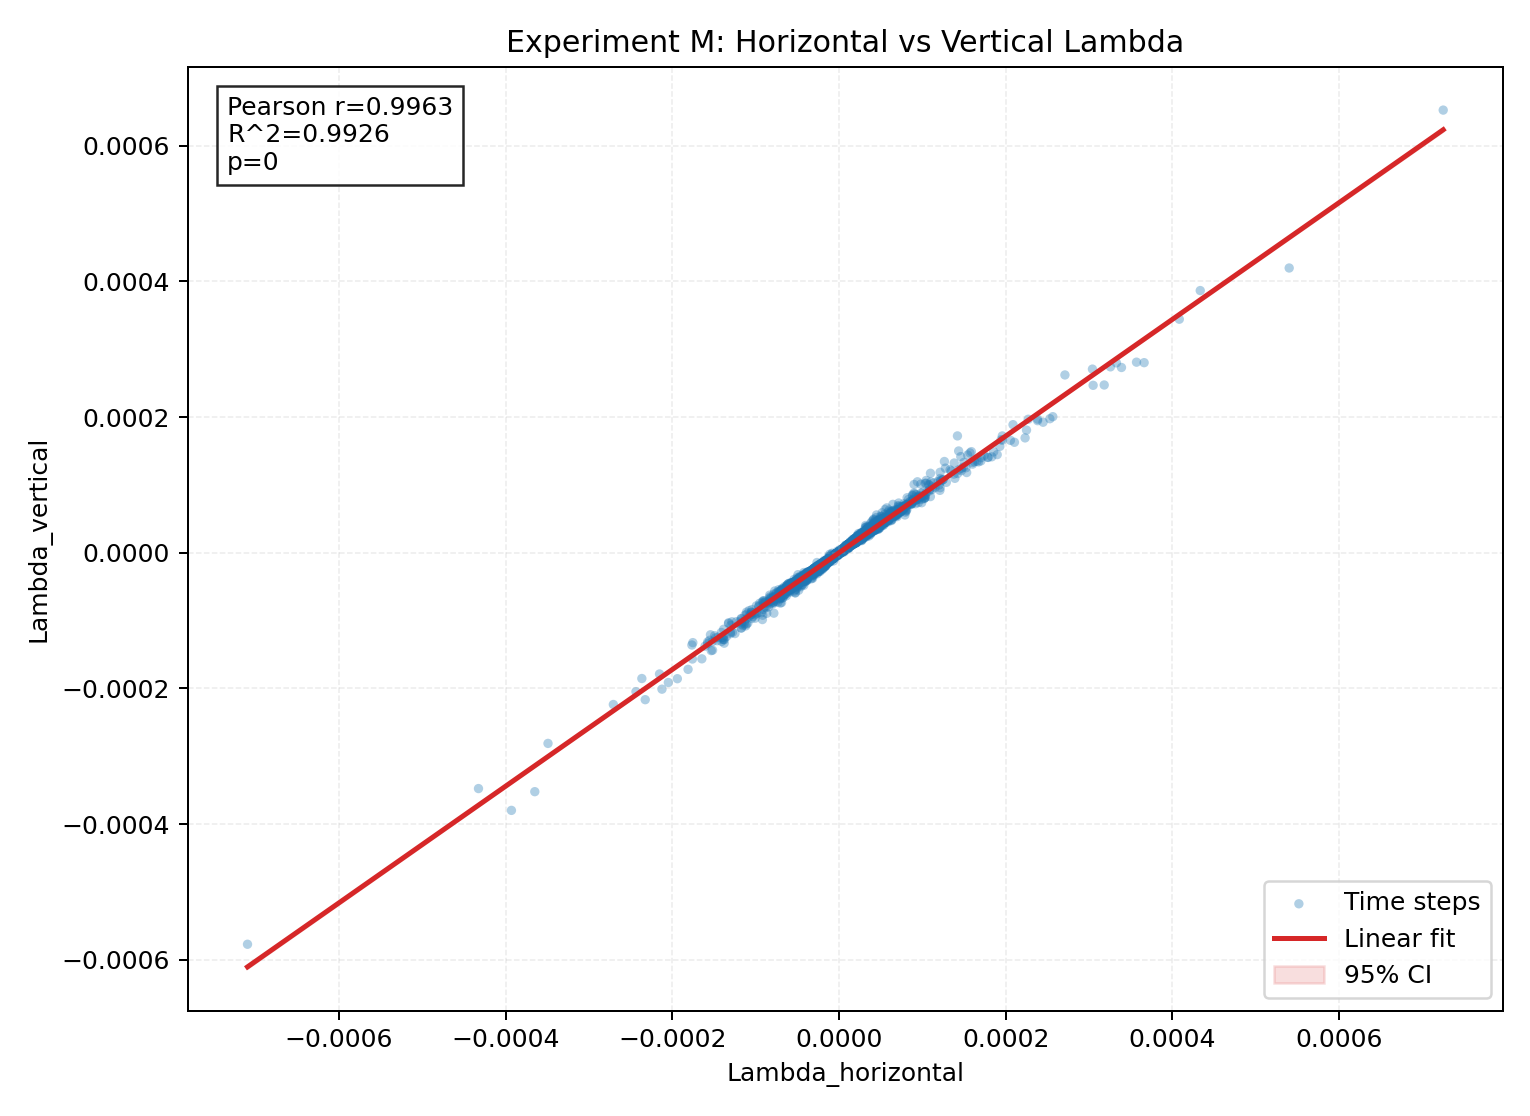
\includegraphics[width=\linewidth]{figures/plot_lambda_scatter.png}
\par\vspace{0.4em}
\small (a) Agreement between predictions $\Lambda_{\mathrm{hor}}$ and $\Lambda_{\mathrm{vert}}$.
\end{minipage}\hfill
\begin{minipage}[t]{0.49\linewidth}
\centering
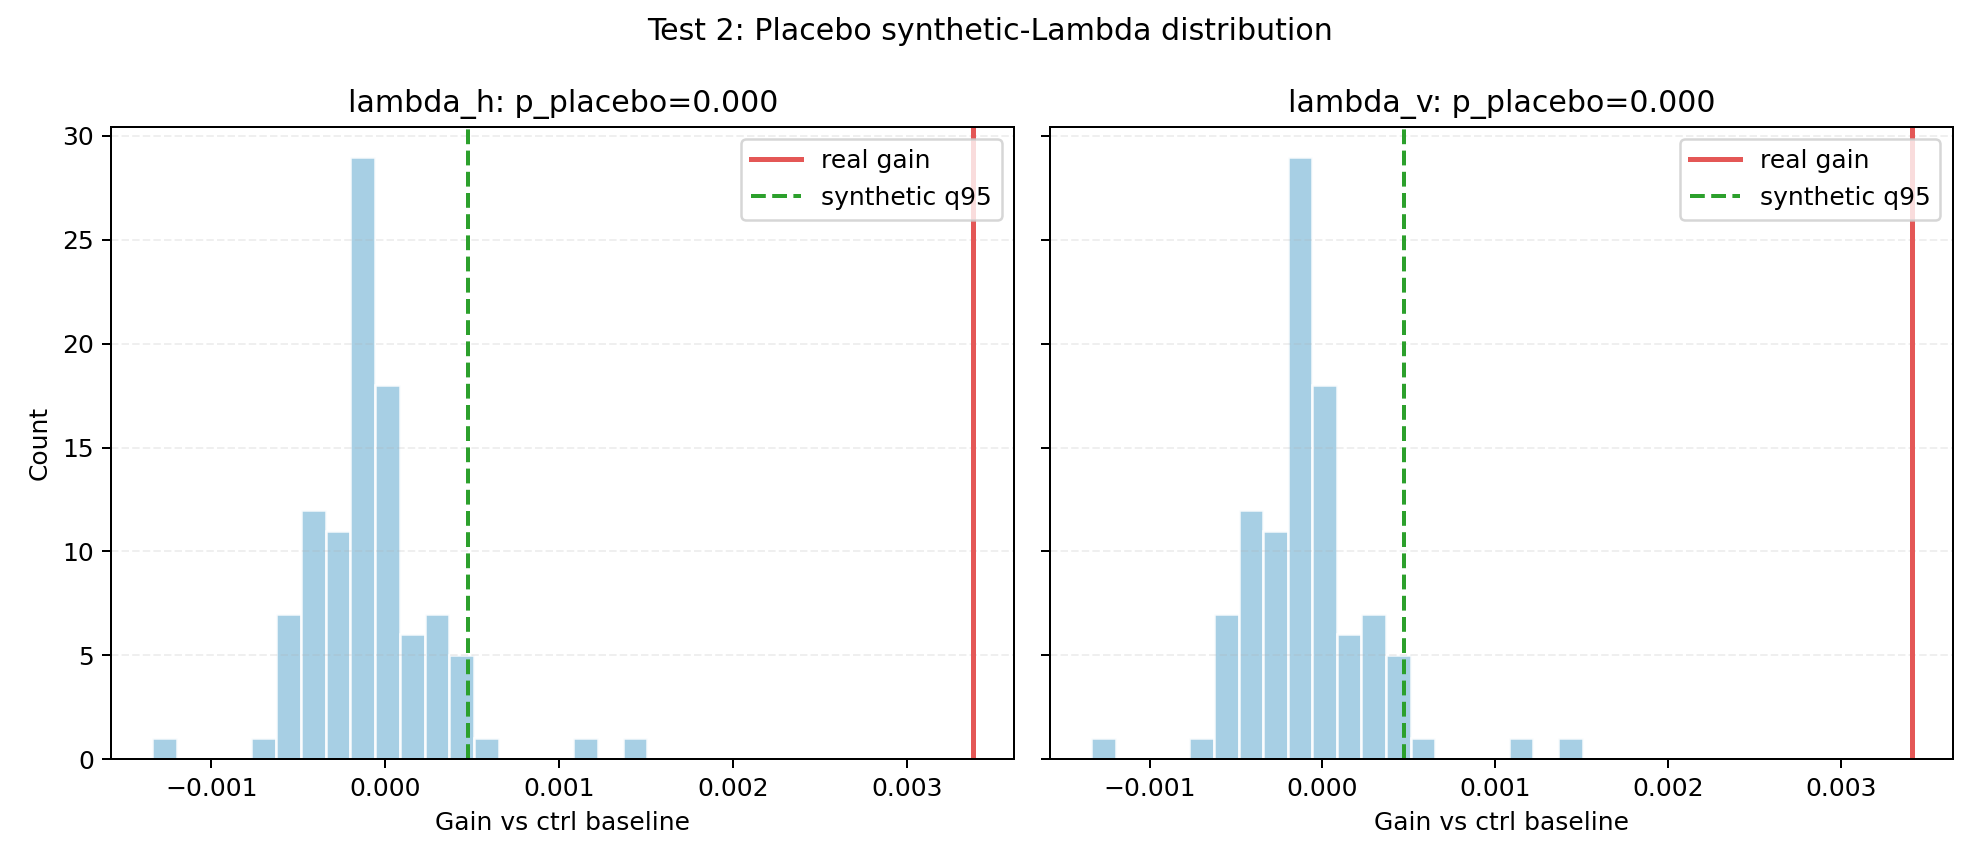
\includegraphics[width=\linewidth]{figures/plot_test2_placebo.png}
\par\vspace{0.4em}
\small (b) OOF-gain distribution for placebo surrogates.
\end{minipage}
\caption{Small but stable macro signal in blocks M1--M2. This block captures observability and structural consistency; direct local closure $\Lambda_b\sim\Pi_b$ is checked separately in A15.}
\label{fig:macro_detectability}
\end{figure}

\subsection{Falsification of necessity controls \texorpdfstring{$\Lambda_{\mathrm{proxy}}$}{Lambda proxy} (M4)}

In the block \texttt{experiment\_M\_lambda\_falsification\_tests} performed three address control of the need \(\Lambda_{\mathrm{proxy}}\)
in the same OOF blocked-CV formulation.

\paragraph{S1: placebo-\(\mu\).}
When rearranging the scale layers,
\[
\Delta_{\mathrm{OOF}}(\Lambda_{\mathrm{real}})=0.003412,\qquad
\Delta_{\mathrm{OOF}}(\Lambda_{\mathrm{placebo\text{-}\mu}})=-0.002986,\qquad
p_{\mathrm{perm}}^{\mathrm{placebo}}=1.0.
\]
Destruction of the interscale structure removes the observed effect and turns the gain into negative area.

\paragraph{S2: \(F^{\mathrm{comm}}\)-control.}
For switching control,
\[
\Delta_{\mathrm{OOF}}(\Lambda_{\mathrm{comm}})=0,\qquad \beta_{\mathrm{comm}}=0,
\]
is obtained, while for \(\Lambda_{\mathrm{real}}\) positive gain is maintained.

\paragraph{S3: information criteria.}
At transition \(\mathrm{ctrl}\to \mathrm{ctrl}+\Lambda_{\mathrm{real}}\) we have
\[
\Delta \mathrm{AIC}=-13.202,\qquad \Delta \mathrm{BIC}=-6.817.
\]
In total, these tests support a narrower, but also more reliable conclusion:
the useful signal is associated precisely with the preserved cross-scale structure, and not with an arbitrary linear addition.

\subsection{Limit of observability: land/ocean, thermodynamic background and spatial diagnostics}

The land/ocean partition captures a characteristic paradox of observability.
In the \texttt{residual\_full} formulation, a positive and significant signal is retained over the ocean
($\Delta_{\mathrm{OOF}}=0.001818$, $p=0.021$),
while gain becomes negative over land
($-0.000491$, $p=0.879$).
Noise-probe shows that a significant part of this difference is due to with a noisier term $P-E$:
in the \texttt{residual\_no\_pe} variant the land-gain practically disappears
($-1.9\times10^{-5}$),
and with 24-hour smoothing \texttt{residual\_full\_roll4} signal restoration is observed on both surfaces
($0.001357$ over land and $0.004099$ over ocean).

Block O1 adds another limitation: on the FT layer the classical Clausius closure is already gives
$R^2_{\mathrm{base}}=0.932165$,
and the addition of $\Lambda_{\mathrm{proxy}}$ changes almost nothing
($R^2_{\mathrm{full}}=0.932161$, $\Delta R^2=-3.75\times10^{-6}$, $p_{\mathrm{perm}}=0.404$).
Accordingly, at the macroscales of the current ERA5 resolution, the interscale correction is either very small or suppressed by the thermodynamic background.

Block O2 confirms the same picture in spatial form:
\[
\mathrm{corr}(\mathrm{gain\_map},\mathrm{convective\_clim})=0.0317,\qquad
\max(\mathrm{gain\_map})=9.20\times10^{-4},
\]
and panel control gives only $3.42\times10^{-6}$ gain.
Therefore, O1--O2 should be interpreted as a diagnostic of the limit of observability, and not as a strong confirmation.

\begin{figure}[t]
\centering
\begin{minipage}[t]{0.49\linewidth}
\centering
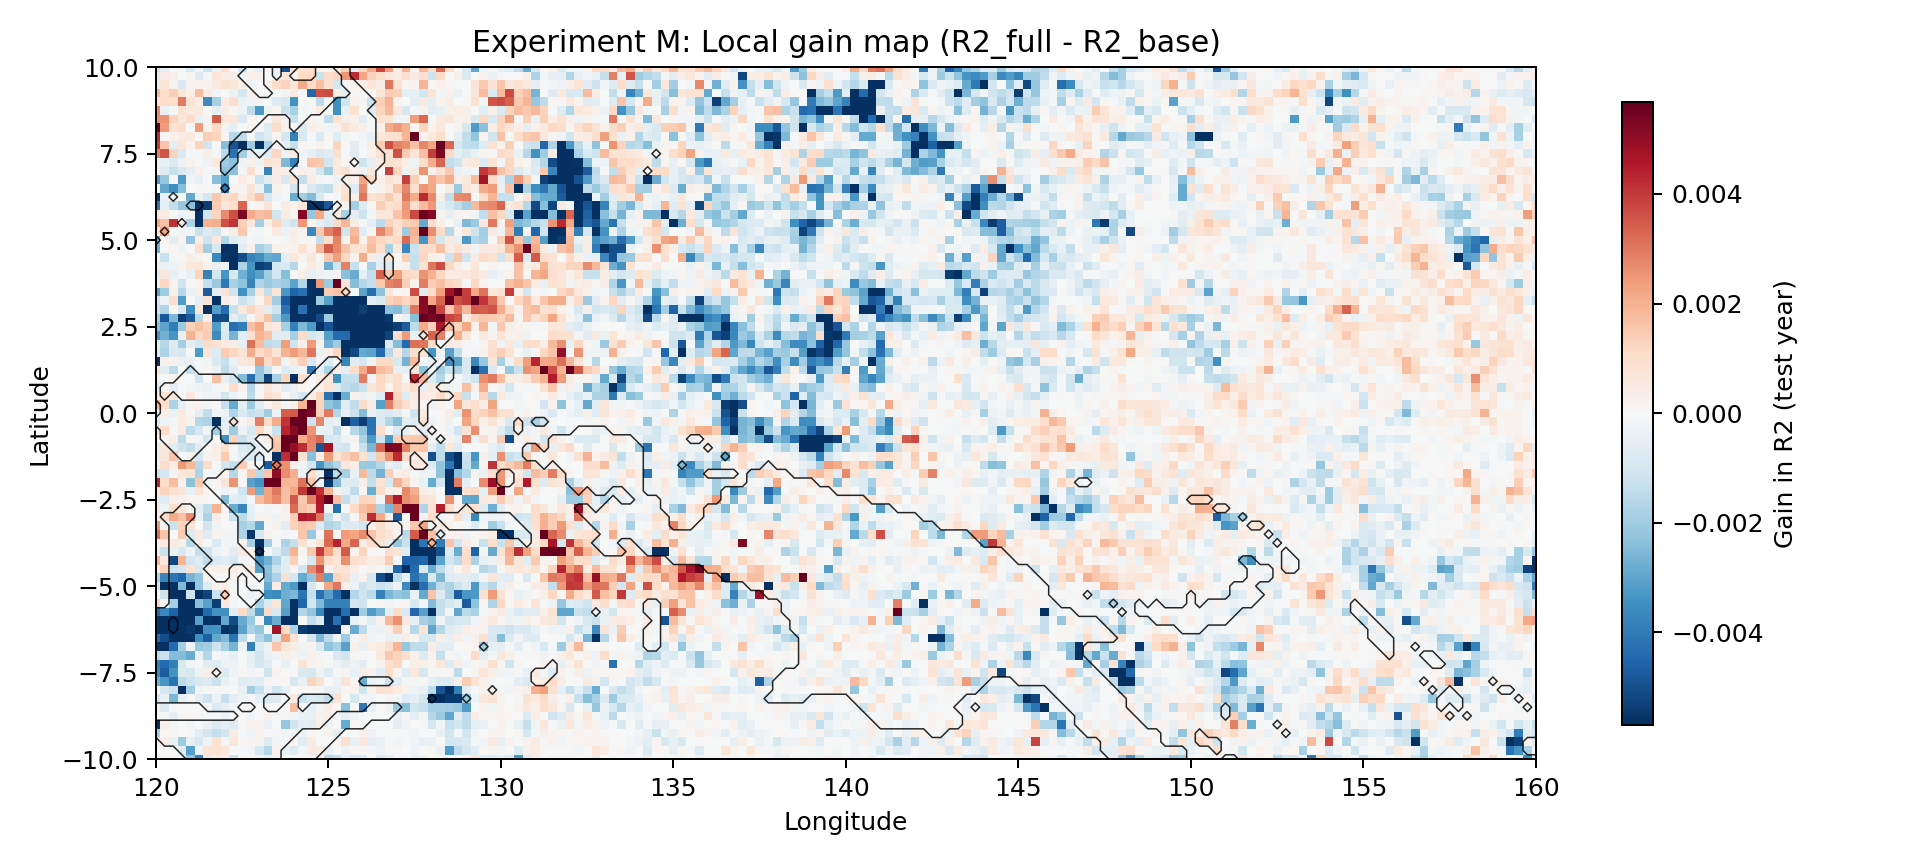
\includegraphics[width=\linewidth]{figures/plot_spatial_gain_map.png}
\par\vspace{0.4em}
\small (a) Local quality gain map $\Delta R^2$ (WPWP, coastline).
\end{minipage}\hfill
\begin{minipage}[t]{0.49\linewidth}
\centering
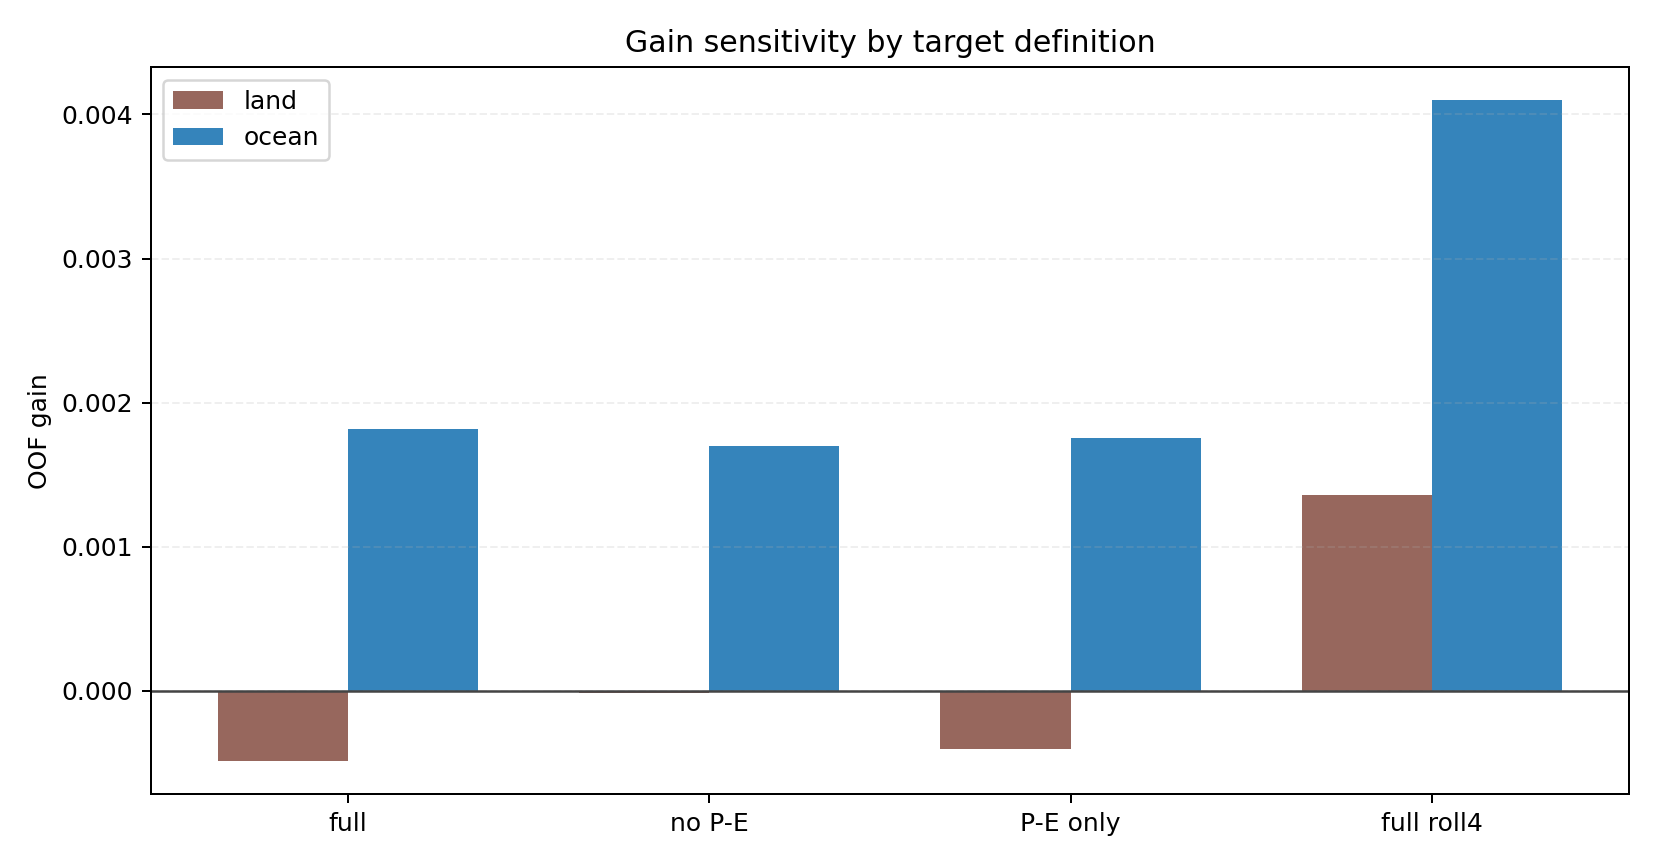
\includegraphics[width=\linewidth]{figures/plot_noise_probe_gains.png}
\par\vspace{0.4em}
\small (b) Median OOF-gain for scenarios \texttt{residual\_full}, \texttt{residual\_no\_pe} and \texttt{residual\_full\_roll4}.
\end{minipage}
\caption{Limit of observability in a macroblock: a positive oceanic signal is adjacent to a regime close to the noise threshold over land and with the dominance of the thermodynamic base approximations.}
\label{fig:macro_noise_limit}
\end{figure}

\subsection{Structural surrogate and tail tests: support and negative results}

The F5 series strengthens the basic M-statement, but also does not give the right to overly strong formulations.
The main observability criterion passes:
\(\Delta_{\mathrm{OOF}}=0.003412\ge 0.002\),
\(p_{\mathrm{perm}}=0.007092\),
\(\mathrm{strata\_positive\_frac}=1.0\).
Two independent fractal surrogates (PSD slope and variogram slope) give a positive relationship with \(\lvert\Lambda_{\mathrm{proxy}}\rvert\)
with correlations of $0.300$ and $0.348$ respectively, but agreement between the surrogates themselves remains moderate
(\(\mathrm{Spearman}=0.587\)).
Consequently, F5 supports a structural, but not definitively unique, interpretation of the signal.

A series of strict tail/SOC tests, on the contrary, in the atmosphere it turns out to be negative.
In F6b for global \(\lvert\Lambda_{\mathrm{local}}\rvert\) a heavy-tail fit is indeed observed,
but the indicator \(\alpha_{\mathrm{emp}}=3.3067\) goes far beyond the pre-announced range of SOC-universality $[1.5,2.0]$.
In F6c, not a single cluster passes the strict corrected test, and in F6c-spatial not a single spatial patch was found,
that simultaneously satisfies the criteria for \(\alpha\), dynamic range, and LLR. That is why in this work we \emph{do not claim} that atmospheric SOC has been confirmed:
the positive model result F6 and the negative atmospheric F6b/F6c/F6c-spatial should be read separately.

\subsection{A05: process-resolved cross-scale bridge and memory on lower layers}

The central new empirical contribution of the manuscript is the A05 series, where the test is transferred
from the macro-averaged ERA5 block to process-resolved setting on individual tiles and panels.
It is here that the formalism gives the most meaningful empirical result:
the scale coordinate turns out to be transferable on sparse and dense panels, but at the finest scale memory is required.

\begin{table}[t]
\centering
\caption{Summary A05.R1--A05.R6. The final memory ladder reads as R3$\to$R6: transfer to a dense panel breaks $l=8$, diagnostics localize the problem to the sensitivity of the fine-scale mode, a minimal short circuit with memory restores the signal, and the full GKSL/CPTP branch shows that the restoration is not a private technical artifact.}
\label{tab:A05_summary}
\small
\begin{tabular}{@{}p{1.4cm}p{4.9cm}p{6.0cm}@{}}
\toprule
Block & What is being tested & Summary \\
\midrule
A05.R1 & Cascade of filling $l\to 2l$ on a sparse panel & ALL: $\mathrm{mae\_gain}=5.10\times10^{-5}$, $\mathrm{R}^2$-gain $=0.0220$; scales $l=8,16$ pass with $\mathrm{perm\_p}=0.02$, and $l=32$ remains borderline. \\
A05.R2 & Calibration of the non-commuting density matrix bridge C009 & Basic C009 selected: overall $\mathrm{mae\_gain}=7.43\times10^{-6}$, $\mathrm{R}^2$-gain $=0.003392$; all scales take place on a sparse panel. \\
A05.R3 & Transfer of C009 to dense intra-event sampling & ALL remains positive ($3.10\times10^{-7}$), $l=16,32$ pass, but $l=8$ degrades: $\mathrm{perm\_p}=0.80$, PASS\_ALL=False. \\
A05.R4 & Narrow-scale failure diagnostics at $l=8$ & Coincident event controls, operator decomposition and mode splitting show that the problem is related to the sensitivity of the fine-scale mode, and not to the composition of the event pool; combo-check gives $\mathrm{mae\_gain}=6.98\times10^{-6}$ and $\mathrm{perm\_p}=0.02$, but remains only diagnostic. \\
A05.R5 & Retarded density matrix memory over fixed C009 & Configuration M001 ($\eta=0.8$, $\tau=0.75$) restores $l=8$: $\mathrm{mae\_gain}=1.22\times10^{-6}$, $\mathrm{perm\_p}=0.02$, event-positive fraction $=0.9375$; all-scale PASS\_ALL=True. \\
A05.R6 & Full GKSL/CPTP memory dynamics over fixed C009 & Configuration G001 gives $l=8$: $\mathrm{mae\_gain}=2.27\times10^{-6}$, $\mathrm{perm\_p}=0.02$, event-positive fraction $=0.9375$; all-scale PASS\_ALL=True, and the CPTP violation proxy is $8.88\times10^{-16}$. \\
\bottomrule
\end{tabular}
\end{table}

The interpretation of this sequence is more important than the individual metrics.
R1--R2 show that the cross-scale bridge in the process-resolved setting is generally detected and transferred.
The final memory ladder then reads R3$\to$R6.
R3 shows that when moving to dense intra-event sampling, the overall signal is not disappears, but it is the instantaneous description on the finest scale that breaks down at $l=8$.
R4 removes the simple explanation through the composition of the event pool: controls for coinciding events leave the gap in place and indicate the sensitivity of the fine-scale mode.
R5 shows that a minimal short circuit with memory is already sufficient to restore portability without removing the quadratic channel and without lowering the standard activity threshold.
R6 repeats this restoration in a stricter full GKSL/CPTP formulation and thereby shows that the effect is not reduced to a specially selected surrogate recipe.

\clearpage
\begin{figure}[H]
\centering
\begin{minipage}[t]{0.92\linewidth}
\centering
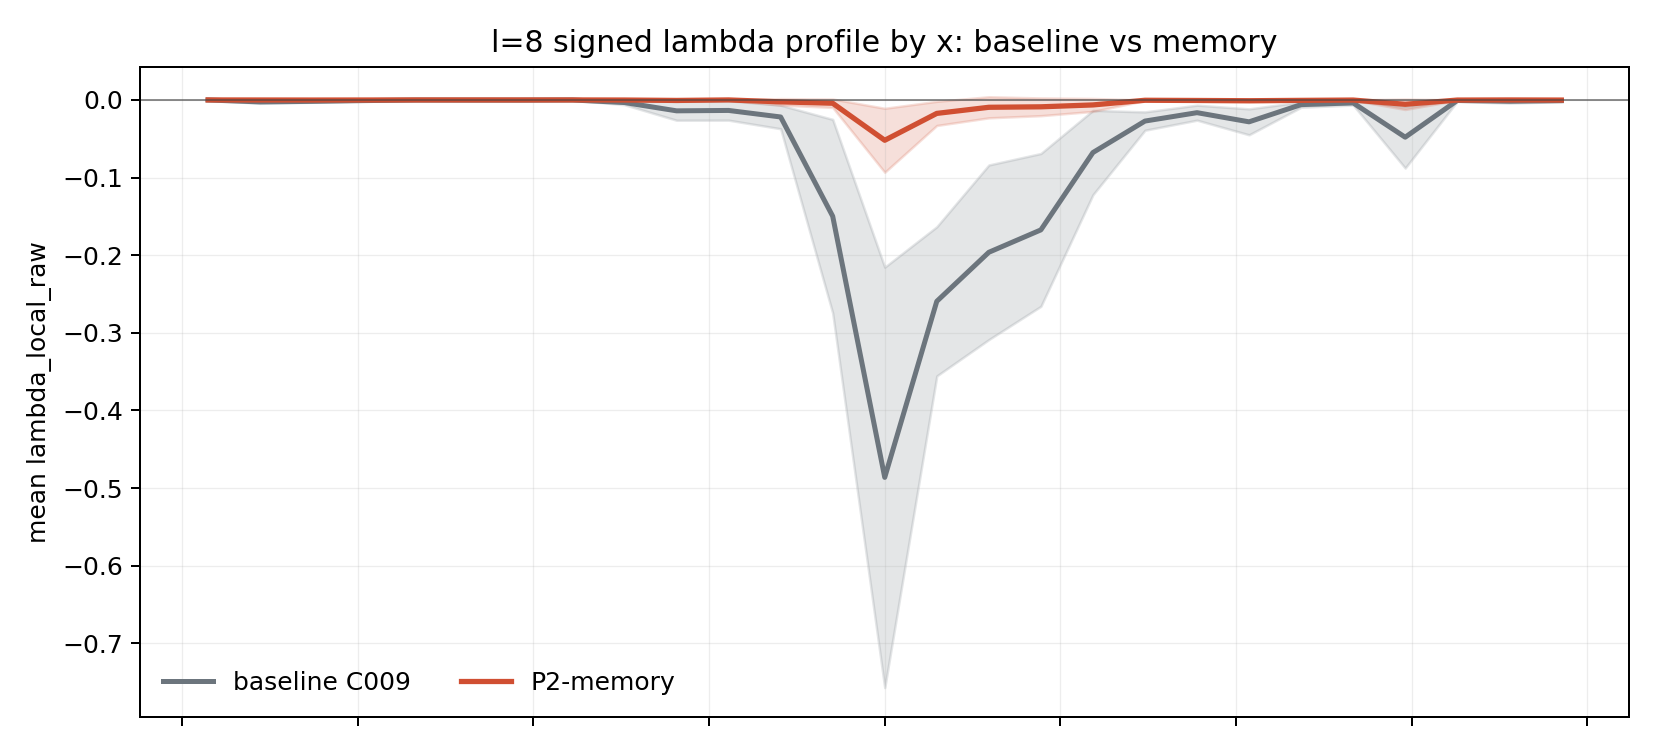
\includegraphics[width=\linewidth]{figures/a05_r5_l8_lambda_profile_baseline_vs_memory.png}
\par\vspace{0.4em}
\small (a) At $l=8$, the memory bridge weakens the negative dip and raises signed $\lambda(x)$ relative to the basic dense scheme.
\end{minipage}

\par\vspace{0.9em}

\begin{minipage}[t]{0.92\linewidth}
\centering
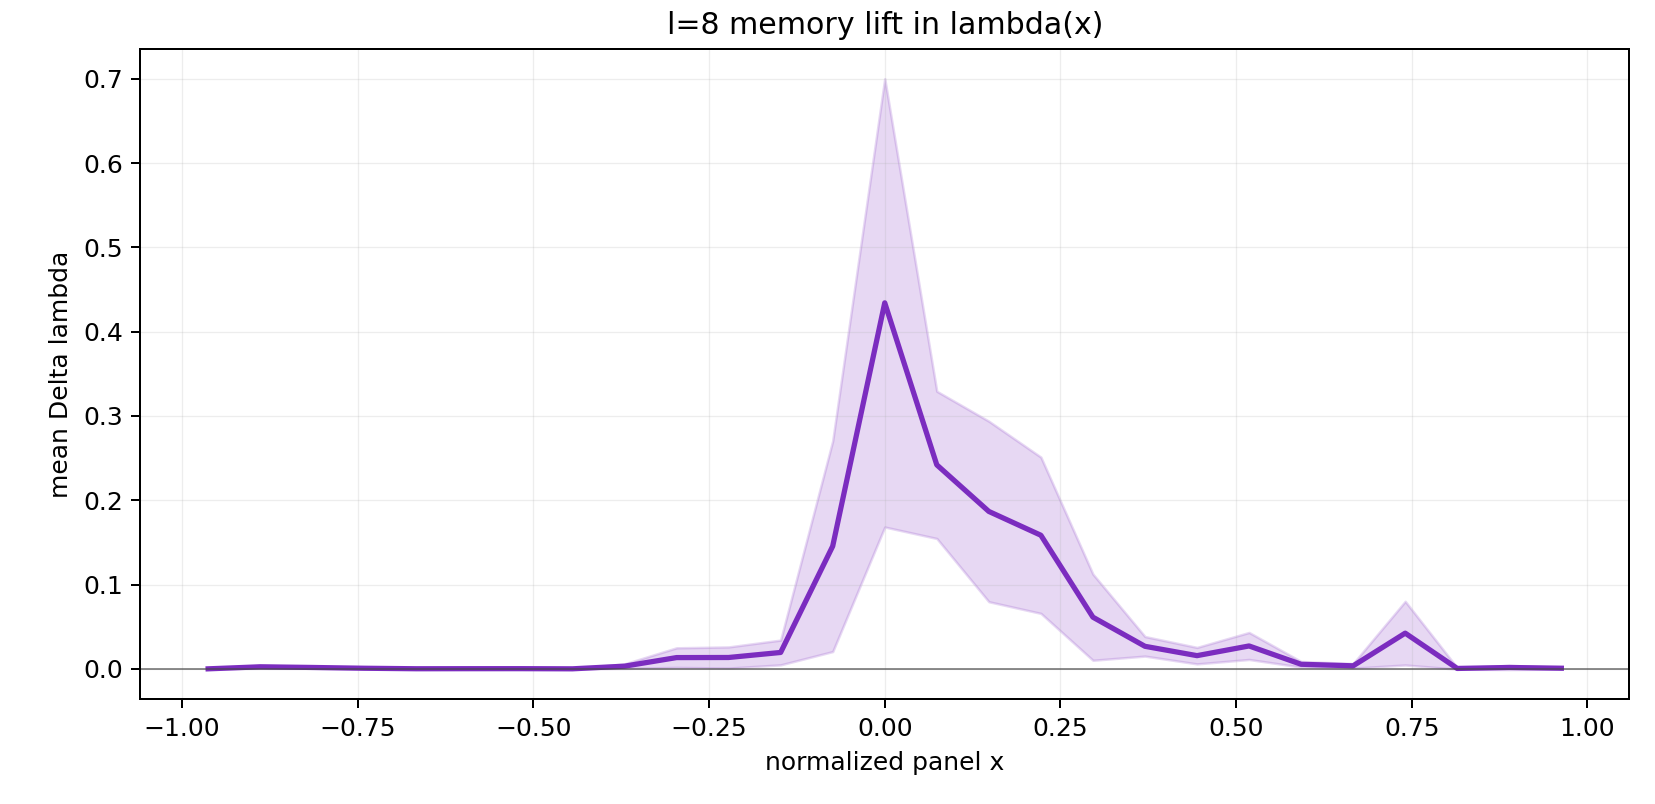
\includegraphics[width=\linewidth]{figures/a05_r5_l8_memory_lift_by_x.png}
\par\vspace{0.4em}
\small (b) Increase in $\Delta \lambda(x)$ is localized in the central $x$-bins and cannot be reduced to a uniform additive shift.
\end{minipage}
\caption{A05.R5: retarded memory of the density matrix as a minimal closure of the finest mode, as close as possible to the formalism. This stage is interpreted as \emph{minimal retarded surrogate}; the more stringent GKSL/CPTP check of R6 is discussed directly in the text below.}
\label{fig:A05_memory}
\end{figure}

R6 completes this branch in a more rigorous physical formulation. In full GKSL/CPTP memory dynamics
configuration G001 gives for $l=8$ $\mathrm{mae\_gain}=2.27\times10^{-6}$ at $\mathrm{perm\_p}=0.02$,
keeps all-scale PASS\_ALL=True and at the same time leaves proxy CPTP violations at the level $8.88\times10^{-16}$.
This is what moves R5 from a successful minimal surrogate to part of a more general reproducible branch of memory.

It is A05 that allows us to formulate the two central empirical theses of the work in a restrained form.
Firstly, the scale coordinate over a fixed $x$ turns out to be operationally meaningful and transferable when modulated.
Secondly, at the smallest scales, a purely Markov instantaneous description turns out to be insufficient:
memory is required to restore the transfer, and this conclusion holds both in the minimal surrogate R5 and in the more rigorous GKSL/CPTP implementation R6.

\subsection[A15: local test Lambda-b--Pi-b closure]{A15: local test Lambda-b--Pi-b closure (``Einstein in the atmospheric column'')}

After the macro- and process-resolved blocks, a direct local test
of the operational \(\Lambda_b\sim\Pi_b\) closure on ERA5 is performed.
The A15 setup uses the wind vector \((u,v)\), scale bands
\([50,100,200,400,800,1600,3200]\) km, sliding window \(W=20\),
operator reconstruction \(\rho_\mu\), \(G_{\mathrm{fwd/back}}\), \(F\), \(\Lambda_b=\Re\Tr(F_b\rho_b)\),
and a proxy for the spectral energy flux
\[
\Pi_b(t)=\left\langle |k|\,E(k,t)\right\rangle_{k\in b},
\qquad
E(k,t):=\frac{|\hat u(k,t)|^2+|\hat v(k,t)|^2}{2}.
\]
On the base ERA5 window
\(2017\text{-}01\text{-}01\;00{:}00{:}00 \ldots 2017\text{-}03\text{-}31\;18{:}00{:}00\)
(360 steps, 6-hour sampling),
the following is obtained:
\[
R^2_{\mathrm{binned,inertial}}=0.520,\qquad
\beta_{\mathrm{inertial}}>0,\qquad
p_{\mathrm{slope}}=0.008.
\]
At the same time, the forcing zone exhibits an inversion/weakening of the slope
(\(R^2_{\mathrm{binned}}=0.179\), negative slope coefficient),
while the dissipation zone shows a decline in fit quality
(\(R^2_{\mathrm{binned}}=0.371\)).
The ERA success criteria for A15 were specified ex ante as
\(R^2_{\mathrm{binned,inertial}}\ge 0.40\), a positive and significant slope coefficient
in the inertial subinterval, together with controlled decay of the relation at the forcing/dissipation edges;
in the base window they are met (\texttt{PASS\_ALL=True}).
Thus, the real atmospheric data captures exactly the regime profile
that is expected for a local scale closure:
operation in the inertial subinterval and controlled decay of coupling at the edges of the cascade.
This provides empirical support for the fact that the gauge-invariant band value \(\Lambda_b\),
constructed from the curvature of connectivity and state, behaves as a geometric proxy quantity,
consistent with the spectral energy flux in the inertial interval.
\begin{figure}[H]
\centering
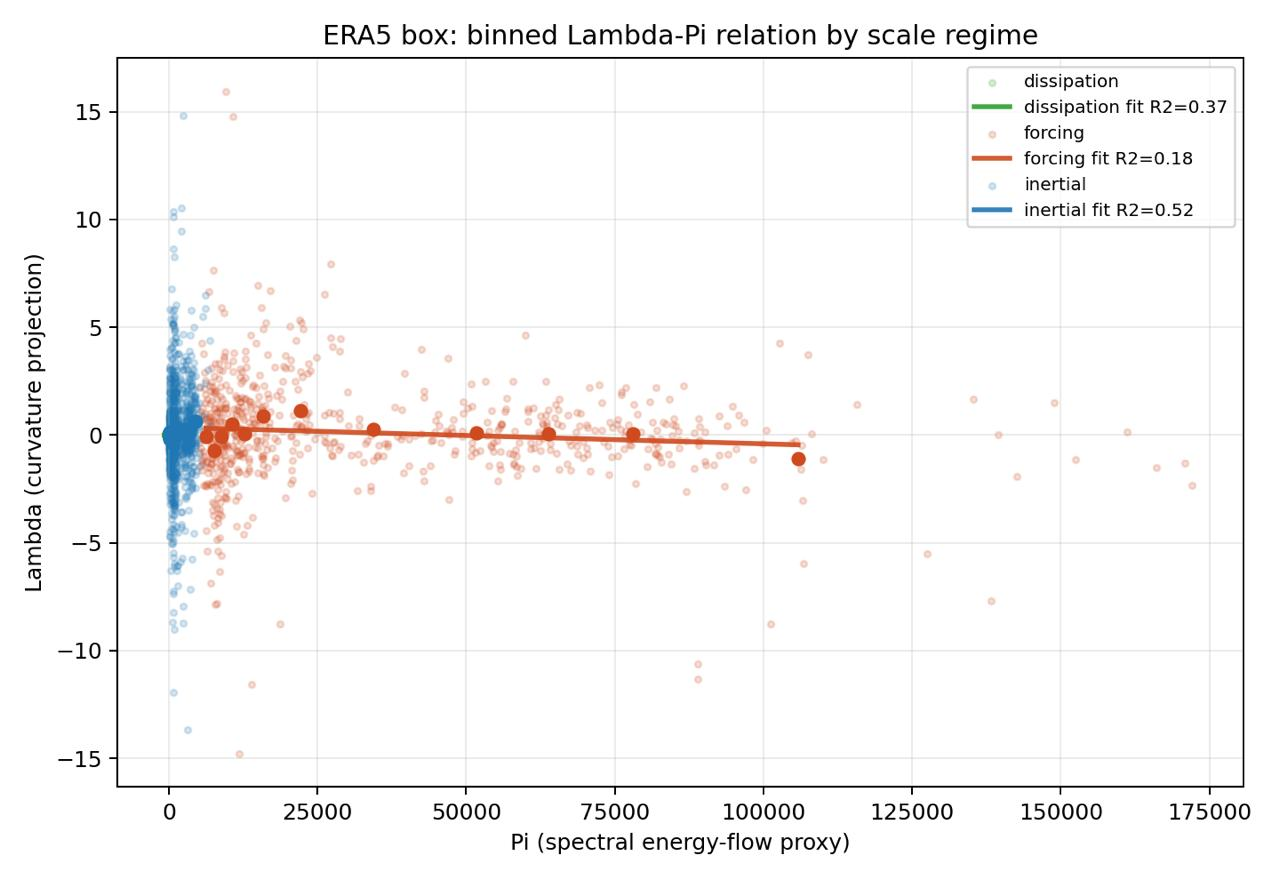
\includegraphics[width=0.9\linewidth]{figures/a15_lambda_vs_pi_regimes.png}
\caption{A15: relation \(\Lambda_b\sim\Pi_b\) by regimes in the ERA5 atmospheric column. In the inertial subinterval, a stable positive dependence is observed, whereas at the cascade edges (the forcing and dissipation zones) the relation predictably weakens or changes sign.}
\label{fig:a15_lambda_pi_regimes}
\end{figure}

\subsection{Limit of local transfer and tests of physically adjacent environment}

The strict chronological test A11, which tested the transfer of the additive $\Phi$ over $\Lambda_{\mathrm{proxy}}$ in the setting training$\le 2019 \rightarrow$ test $2020 \rightarrow$ external control $2021$, gives a negative result. For the control year 2020, we get $\Delta_{\Lambda_{\mathrm{proxy}},\mathrm{ctrl}}=-0.002240$ at $p=0.4055$, and adding $\Phi$ on top of $\Lambda_{\mathrm{proxy}}$ gives only $\Delta_{\Phi,\Lambda_{\mathrm{proxy}}}=-0.000067$ at $p=0.3810$; at external 2021 $\Delta_{\Phi,\Lambda_{\mathrm{proxy}}}=-0.000023$ remains at $p=0.3350$. In other words, the transfer of local closure on one tile does not demonstrate stable generalization in a strict formulation of the forecast for the year ahead.

Block A12 removes this limitation by introducing a physically adjacent boundary environment when estimating only from the inner kernel. Here the \texttt{ERA\_window} model dramatically outperforms \texttt{ERA\_core}: the gain is $0.136707$ on the 2020 test and $0.092229$ on the 2021 external control, in both cases with $p=0.0005$. The increases from $\Phi_H$ and $\Lambda_H$ over this window are small, so the main effect is associated precisely with the presence of a physically adjacent environment.

Block A13 refines this conclusion by scanning the width of the boundary ring. At $w=0$ the gain disappears, and the maximum is reached at $w=4$: $0.151703$ on the test and $0.156626$ on the external control; at $w=6,8,10$ the effect remains positive, but consistently weakens. Consequently, we are not talking about the usefulness of an arbitrarily expanded set of features, but about the local and non-monotonic scale of boundary interaction.

Block A14 completes the series with a falsified comparison of a physically adjacent environment with a distant and displaced one. For a fixed $w=4$, the local environment confidently outperforms both controls: \texttt{local} gives $0.151703/0.156626$, while \texttt{remote} --- $0.097182/0.058412$, and \texttt{misaligned} --- $0.073343/0.059724$ on test and external control, respectively. This means that it is the physically adjacent environment that is essential for atmospheric transport, and not any additional external signal.

\paragraph{Limits of interpretation of the atmospheric block.}
Current atmospheric data are too coarse to identify the complete internal structure of the $\Lambda_{\mathrm{matter}}$ object and its stripe projections from the formal model.
However, they are sufficient to test whether the observed patterns predicted by the formalism persist after coarse-graining and measurement constraints, including the direct coupling of $\Lambda_b\sim\Pi_b$ in the inertial interval.
The strongest empirical results of this section now include: (i) a direct local test of \(\Lambda_b\sim\Pi_b\) in A15, (ii) the role of memory in A05.R5--R6, (iii) dependence on the physically adjacent boundary environment in A12--A14. Thermodynamic and SOC-related signals remain secondary and limited in output strength.

\begin{table}[H]
\centering
\caption{Synthetic summary of block A12--A14.}
\label{tab:A12_A14_summary}
\small
\begin{tabular}{@{}p{2.8cm}p{3.9cm}p{4.0cm}p{4.0cm}@{}}
\toprule
Question & Protocol & Main result & Interpretation \\
\midrule
A12: Is a physical neighborhood necessary? & Estimated by the inner core by adding a boundary ring around it; strict transfer of training$\le 2019 \rightarrow 2020 \rightarrow 2021$. & \texttt{ERA\_window} gives $0.136707/0.092229$ relative to \texttt{ERA\_core}; the additions $\Phi_H$ and $\Lambda_H$ are small. & The key benefit is created by the physically adjacent environment itself. \\
A13: What is the characteristic width of the environment? & Fixed core placement and width scanning $w\in\{0,4,6,8,10\}$. & The maximum is reached at $w=4$: $0.151703/0.156626$; at large $w$ the effect becomes saturated and weakens. & The boundary effect is local and non-monotonic in width. \\
A14: Is the neighborhood important? & When $w=4$, local, remote and displaced environments are compared with the same kernel metric. & \texttt{local} outperforms \texttt{remote} and \texttt{misaligned}: $0.151703/0.156626$ vs. $0.097182/0.058412$ and $0.073343/0.059724$. & It is the physically neighboring environment that is essential, and not arbitrary external information. \\
\bottomrule
\end{tabular}
\end{table}

The final logic of the section is as follows: A11--A14 set the limit of transferability of local reduction and show the decisive role of the physically neighboring environment, and A15 gives the most rigorous and direct empirical result of the entire atmospheric part --- local verification \(\Lambda_b\sim\Pi_b\) in the inertial interval ERA5 (see\ \cref{fig:a15_lambda_pi_regimes}).

\paragraph{Reproducibility (empirical block).}
The canonical set of core scripts for the empirical block is published in the active release:
\url{https://github.com/Theclimateguy/Shroedinger/releases/tag/v2.1}.
Heavy intermediate/final artifacts and continuation runs (A05.R* and A07.R*) are preserved as separate runtime downloads and are not included in the compact package by default.

% =========================================================
\section{Discussion: what is supported, what remains a hypothesis}
\label{sec:discussion}

\paragraph{Which is supported by current data.}
At the level of model validation, the formalism looks internally consistent:
the gauge invariants are stable, the balance on $(t,x,\mu)$ is closed,
and blocks F1--F6 together with T20 show that within one numerical class it is possible to sequentially associate the balance mode,
scale covariance, fractal proxies, holonomy and model SOC.
At the atmospheric level, support has also become more direct:
M1--M4 give a weak and reproducible structural signal in the closure task,
and A05.R3--R6 gives a complete memory ladder: transfer to a dense panel breaks exactly $l=8$,
diagnostics relate this failure to fine-scale mode sensitivity, a minimal short circuit to memory restores the signal,
and a more rigorous GKSL/CPTP implementation confirms that the restoration is not a proprietary technical artifact.
The key addition A15 provides direct empirical support for \(\Lambda_b\sim\Pi_b\) in the ERA5 inertial range
(\(R^2_{\mathrm{binned}}=0.520\), \(p=0.008\)) together with the expected decay of the relation in the forcing/dissipation ranges.

\paragraph{Local atmospheric reduction limit.}
A05.R6 shows that the physics of memory at the finest scale remains viable in a process-resolved setting: recovery is maintained not only in the minimal surrogate, but also in the full GKSL/CPTP dynamics. At the same time, block A11--A14 shows the limit of applicability of a more stringent local atmospheric reduction: transfer on one tile does not generalize stably in the year-ahead setting, whereas the physically adjacent environment yields a large and reproducible gain. A15 completes this picture as the strongest empirical foundation: the local $\Lambda_b\sim\Pi_b$ closure is maintained in the local-cell regime, but remains mode-dependent when the window and the external dynamical regime change.

The next natural step is therefore not another local ablation, but the construction of a more complete atmospheric model of the open system, where the environment of the local subsystem is given explicitly. At the level of formulation, this indicates the need to move from a single slab to a quasi-global or, in the limit, a holistic atmospheric configuration with controlled interscale and interregional exchange.

\paragraph{Which is not yet supported.}
The same data do not allow us to draw stronger conclusions.
We have not established the physical status of $\Lambda_{\mathrm{matter}}$ as a fundamental constant;
it remains an effective source and diagnostic proxy term.
We have not derived a first-principles thermodynamic closure for the entire real atmosphere:
O1--O2 and the window dependence in A15 show that outside the local-cell regime and without explicit treatment of the mode structure,
the signal may weaken substantially.
Finally, we do not confirm the universal atmospheric SOC mode:
strict tail and F6b/F6c/F6c-spatial cluster tests remain negative.

\paragraph{Operational findings and strong interpretations are not the same thing.}
Most a reliable operational result of the work is that the scale coordinate is useful as a description variable
and that at the lower layers memory is required, and at the atmospheric level the local subsystem is sensitive to the physically neighboring environment.
R6 strengthens the first conclusion, and A12--A14 --- the second.
But this is still not identical to the statement of a complete non-Markovian theory of nature, does not prove a universal one 5D geometry
and does not eliminate the need for a separate output of dynamics with memory and an explicit model of the environment.
We consider this difference to be fundamental for fair positioning of the result.

\paragraph{Connection with close directions.}
The proposed frame naturally comes into contact with RG geometry and local RG
\cite{Zamolodchikov1986Irreversibility,Osborn1991LocalRG,CotlerRezchikov2023RGOptimalTransport},
with information geometry and holonomy of quantum channels
\cite{Amari2016InformationGeometry,Uhlmann1986QuantumHolonomy,KultAbergSjoqvist2008HolonomyChannels},
as well as with thermodynamic gravity in the spirit of Jacobson
\cite{Jacobson1995EinsteinEOS,ElingGuedensJacobson2009NonEq}.
The difference in our work is that these ideas are used as working guidelines for the program being tested,
and not as an already closed fundamental conclusion.

\section{Limitations and further work}
\label{sec:limitations}

Within declared level (local scale-thermodynamic closure in the cell), the theory is closed in the operational sense: T20 and A15 provide direct empirical support for the connection \(\Lambda_b\sim\Pi_b\) in the inertial interval.
When going beyond this level, open questions remain.
More strictly, the internal geometric core of the scale cell can be closed as a local variational model: the projector field \(P_*(s,\mu)\) can be generated by a CP1/O(3)-type action on a two-dimensional base \((s,\mu)\), after which the connection \(A_i\), curvature \(F_{ij}\), and a local object of the form \(\mathrm{Tr}(\rho F)\) are no longer free quantities.  However, this is not a complete fundamental derivation: such an internal cell does not by itself fix the absolute KMS relaxation-rate scale, the normalization of \(T_{\alpha\beta}^{\mathrm{scale}}\) under metric variation, or the physical source map \(\rho_{\mathrm{phys}}\mapsto(s,\Delta,\beta)\).  Thus the claims of this paper should be read as a local operational and model-geometric closure, not as a completed theory of the gravitational source.
The memory branch in A05 now includes both the minimal surrogate R5 and the more stringent GKSL/CPTP implementation of R6. This significantly strengthens the physical consistency of the result, but still does not replace the general conclusion of non-Markovian dynamics with a historical kernel derived from first principles.
The thermodynamic block in the local mode is supported empirically, but this is not equivalent to the universal first-principles derivation for the full atmosphere or the general quantum field system.
The atmospheric signal remains mode-dependent. In addition to WPWP/ERA5 and the canonical A05 panel, the strict block A11--A14 shows that the transfer of local closure on one tile is unstable, and the reproducible gain occurs only when the physically adjacent environment is explicitly taken into account. Frozen-extensions A07.R1--A07.R5 (see \hyperref[sec:appendix:atmo]{Appendix~A.3}) strengthen this conclusion: in independent extensions, some runs remain negative or borderline. This highlights the need for independent geographic and seasonal replicates without retuning.
For stronger conclusions, the following classes of data are needed: denser process-resolved panels, LES/CRM level for direct testing of thermodynamics at the smallest scales, and independent regions and seasons with a pre-fixed protocol.
The physical status of $\Lambda_{\mathrm{matter}}$, the universality of the thermodynamic closure, and a possible connection with a broader fundamental theory remain open.


\section{Conclusion}
\label{sec:conclusion}

The paper proposes a formalism of scale geometry on an extended base $(x,t,\mu)$ with covariant dynamics and consistent coarse-graining.
In controlled model experiments, the formalism undergoes internal validation (gauge consistency, balance, bridges and structural checks) and leads to a constructively defined observable $\Lambda_{\mathrm{matter}}$ and its band-pass version $\Lambda_b$.
At the model stage T20, a stable connection \(\Lambda_b\sim\Pi_b\) is observed in the inertial range, and in the atmospheric block A15 empirical support for the same local dependence was obtained on ERA5 data. This result is consistent with the thermodynamic interpretation of geometric closure, but applies specifically to the controlled mode of the local cell.

The strongest empirical results of the paper relate to three nodes of the program: the role of memory at fine scales (A05.R5--R6), local $\Lambda_b\sim\Pi_b$-closure (T20/A15) and the physically adjacent boundary environment (A12--A14). Together they provide not a universal theory, but a consistent and reproducible operational set of consequences of the formalism.

The resulting picture supports a thermodynamic-geometric reading of the model, but does not resolve open questions about the fundamental status of $\Lambda_{\mathrm{matter}}$, the universality of closure outside the local cell, and memory derivation by first principles.

The final logic of the manuscript remains hierarchical:
formalism, then controlled validation, then empirical tests of rough consequences, then the limits of applicability and further steps.

% =========================================================
\appendix
\newpage

\phantomsection
\section*{Appendix C. Glossary of terms and abbreviations}
\addcontentsline{toc}{section}{Appendix C. Glossary of terms and abbreviations}
\label{sec:appendix:glossary}

\subsection*{C.1 Abbreviations}

\begin{table}[H]
\centering
\caption{Main abbreviations in text.}
\label{tab:appendix_c_abbr}
\small
\begin{tabular}{@{}p{2.8cm}p{11.2cm}@{}}
\toprule
Abbreviation & Brief Explanation \\
\midrule
ERA5 & ECMWF Global Atmospheric Reanalysis (multi-year consensus archive of atmospheric fields). \\
WPWP & Tropical moisture budget pilot as part of an ongoing set of experiments. \\
OOF & \textit{Out-of-fold}: testing on data fragments that were not involved in training at this step. \\
GKSL & Equation of open quantum dynamics (Gorini--Kossakowski--Sudarshan--Lindblad). \\
CPTP & Class of mappings that preserve the physicality of the state: complete positivity and trace preservation. \\
SOC & Self-organized criticality (power-law tail regime in systems with slow supply and sharp discharges). \\
RG & Renormalization group evolution by scale. \\
LES/CRM & Highly detailed classes of atmospheric modeling (large-eddy and cloud-resolving). \\
MRMS/GOES & High resolution observation sets (radar and satellite channels). \\
\bottomrule
\end{tabular}
\end{table}

\subsection*{C.2 Key Terms in Plain Language}

\begin{table}[H]
\centering
\caption{Terms important for interdisciplinary reading.}
\label{tab:appendix_c_terms}
\small
\begin{tabular}{@{}p{3.6cm}p{10.4cm}@{}}
\toprule
Term & Explanation without highly technical details \\
Hamiltonian $H$ & Operator that specifies the ``move rule'' of a system in time: what states change and how quickly. \\
\midrule
Hilbert space & Linear state space with inner product; in operation it is a ``container'' for the state at each scale. \\
Hilbert bundle & A family of such spaces over points $(x,t,\mu)$: each position and scale has its own layer of states. \\
Density matrix $\rho$ & A way to describe not only a ``pure'' state, but also a mixture of states and incomplete information about a system. \\
Coherence & Off-diagonal elements $\rho$; characterize the consistency of phases between the components of the state. \\
Gauge connectivity $A_M$ & Rule for how to consistently transfer states and operators between adjacent points/scales; specifies the ``translation geometry''. \\
Gauge invariance & The requirement that the physical output is independent of the chosen local basis (``coordinate system'' in internal space). \\
Scale connectivity $A_\mu$ & Operator describing the transfer of information between adjacent scales. \\
Curvature $F_{\mu\nu}$ & Measure of non-commutativity of translations; Invariant diagnostic scalars are constructed from it. \\
Holonomy & Integral effect of transfer along a closed loop: after traversing the loop, the state can return with a non-trivial ``turn''. \\
Causal Diamond & Local region of space-time defined by the intersection of future and past light cones; used as a small domain for local thermodynamic estimates. \\
Local horizon & Causal accessibility boundary for the selected local observer; through it, the thermodynamic route takes into account the flow of energy. \\
Modular generator & Operator $K=-\log\rho_{\mathrm{ref}}$, encoding the structure of the local reference state; in the small diamond is associated with the boost flow. \\
Detailed balance & Consistency condition of dissipative dynamics with the local reference state; ensures non-negative entropy production. \\
Holographic clipping (screen) & Practical limitation of the number of degrees of freedom according to the ``boundary'' rule to control the growth of the model dimension while maintaining the basic structure. \\
Coarse-graining the scale & Transition from a more detailed description to a larger (averaged) one without violating the physical correctness of the state. \\
Markov limit & Approximation without ``memory'' of the past: the next state depends only on the current one. \\
Memory (non-Markovianity) & A situation where past states significantly influence the current dynamics. \\
Falsification control & Special test that should destroy the effect if it is caused by an artifact and not by the structure of the model. \\
Boundary environment (halo) & Physically adjacent area around the forecast core; in the article, this is a key factor in improving closure. \\
\bottomrule
\end{tabular}
\end{table}

\phantomsection
\section*{Appendix T. Theoretical and model validation}
\addcontentsline{toc}{section}{Appendix T. Theoretical and model validation}
\label{sec:appendix:toy}

\subsection*{T.0 Complete derivation of Einstein's thermodynamic route}
\label{sec:appendix:einstein_full}

\paragraph{Status of this appendix.}
Below is the complete technical route, which in the main text has been reduced to the final formula.
This route is retained as an interpretative and verification tool for the consistency of the formalism,
but is not used as the main empirical one output.

\paragraph{Step 1: modular generator of local reference state.}
For a small causal diamond $\Omega$ we set
\begin{equation}\label{eq:app_modular_state}
\hat\rho_{\Omega}^{\mathrm{ref}}
=
Z_\Omega^{-1}\exp\!\left(-\hat K_{\Omega}^{\mathrm{mod}}\right),
\qquad
\hat K_{\Omega}^{\mathrm{mod}}:=-\log \hat\rho_{\Omega}^{\mathrm{ref}}.
\end{equation}
In a discrete implementation:
\begin{equation}\label{eq:app_modular_discrete}
\hat K_{\Omega}^{\mathrm{mod}}
=
\sum_{i\in\Omega}\kappa_i h_i,
\qquad
\kappa_i=-\log p_i^{\mathrm{ref}}.
\end{equation}

\paragraph{Step 2: local ``first law'' of relative entropy.}
Using (A1)--(A3) and \cref{eq:entropy_production_local}, we get
\begin{equation}\label{eq:app_firstlaw_mod}
\delta S_{\mathrm{hor}}
=
\delta\!\left\langle K_{\Omega}^{\mathrm{mod}}\right\rangle
+O(\varepsilon^2).
\end{equation}
Identification of energy flow through balance \cref{eq:balance} leads to local form
\begin{equation}\label{eq:app_clausius}
T_\ast\,\dd S_{\mathrm{hor}}
=
\delta Q_{\mathrm{in}}
=
\int_{\partial\Omega}T_{ab}\chi^a\,\dd\Sigma^b
+O(\varepsilon^2).
\end{equation}

\paragraph{Step 3: small diamond limit and boost generator.}
At (A5) modular flow asymptotically turns into local boost flow:
\begin{equation}\label{eq:app_boost_limit}
\hat K_{\Omega}^{\mathrm{mod}}
=
\hat K_{\Omega}^{\mathrm{boost}}
+O\!\left(\frac{\xi(\mu)^2}{\ell_\Omega^2}\right).
\end{equation}
Thereby, the boost structure arises as a limiting form of modular locality, and is not entered manually.

\paragraph{Step 4: final limit.}
The combination \cref{eq:arealaw,eq:app_clausius,eq:app_boost_limit} gives
\begin{equation}\label{eq:app_einstein_full}
G_{ab}+\Lambda g_{ab}
=
8\pi G_{\mathrm{eff}}(\mu)\,\langle T_{ab}\rangle
+O(\varepsilon^2)
+O\!\left(\frac{\xi(\mu)^2}{\ell_\Omega^2}\right),
\end{equation}
which coincides with the form, given in the main text (\cref{eq:deriv_einstein}).

\paragraph{Conditions of applicability and limitations.}
The derivation requires a quasi-static regime, locality of correlations and correctness of the balance identification of heat flow.
Outside these conditions, nonequilibrium corrections are required (in the spirit \cite{ElingGuedensJacobson2009NonEq}) and an explicit memory/environment model.
The connection with 5D projections and braneworld geometry in \cref{rem:5d_bridge} remains interpretive,
and not the only possible reduction.
Empirically in this article, the route gets a local support in the cell (T20/A15) through the connection \(\Lambda_b\sim\Pi_b\) in the inertial interval, but does not close as a universal thermodynamic-gravitational output for the entire atmosphere.

\subsection*{T.1 Minimum implementation checks}

\begin{table}[H]
\centering
\caption{Basic checks of the implementation of the formalism.}
\label{tab:appendix_t_impl}
\small
\begin{tabular}{@{}p{4.8cm}p{4.1cm}p{5.1cm}@{}}
\toprule
Verification & Metrics & Result \\
\midrule
Translation unitarity and cocycle & $\|U^\dagger U-I\|_F$, $\|U_{23}U_{12}-U_{13}\|_F$ & $1.77\times10^{-16}$ and $3.34\times10^{-16}$ \\
Isometricity of embedding & $\|V^\dagger V-I_2\|_F$ & $0$ \\
Lindblad structure and trace conservation & $\max(\|{\rm anti}(H_{\rm eff})+i\dot\mu A_\mu\|_F,|\Tr\dot\rho|)$ & $5.55\times10^{-17}$ \\
Classical limit $\dot\mu\to 0$ & $\max|\Delta\Re\lambda|$, $\max|\Im\lambda|$, $\|H_{\rm eff}-H_\mu\|_F$ & $1.14\times10^{-9}$, $2.10\times10^{-5}$, $6.02\times10^{-5}$ \\
Finiteness of curvature and Bianchi identity & $\|F_{12}\|_F$, Bianchi remainder & $\|F_{12}\|_F=4.18\times10^{-1}$, remainder $1.96\times10^{-17}$ \\
Total preservation of the norm across layers & $\max_t|(\|\Psi_{\mu_1}\|^2+\|\Psi_{\mu_2}\|^2)-1|$ & $9.50\times10^{-14}$ \\
\bottomrule
\end{tabular}
\end{table}

\subsection*{T.2 Map of model blocks T01--T20}

{\small
\begin{longtable}{@{}p{1.1cm}p{3.2cm}p{5.1cm}p{3.8cm}@{}}
\caption{Summary map of model experiments.}\label{tab:appendix_t_map}\\
\toprule
Code & Block & Main result & Limitation / status \\
\midrule
\endfirsthead
\toprule
Code & Block & Main result & Limitation / status \\
\midrule
\endhead
T01 & Gauge invariance & All gauge checks passed; $\max|\Delta\Lambda_{\mathrm{matter}}|\sim10^{-15}$. & Finite-dimensional model sector, not full QFT. \\
T02 & Two-layer $\mathfrak u(2)$-control & Sinusoidal law and state-dependence pass in all $120/120$ cases. & Restricted to the $\mathfrak u(2)$-class. \\
T03 & Balance at $(t,x,\mu)$ & Balance balance $\sim4.44\times10^{-16}$. & Discrete formulation and model operators. \\
T04 & Coherence vs. $|\Lambda_{\mathrm{matter}}|$ & Coherence systematically better predicts vertical dynamics: average $\Delta R^2\approx0.048$. & Synthetic trajectories, not analytical inference. \\
T05 & Robustness of the sinusoidal law & Maximum relative error $6.29\times10^{-15}$. & Restricted family of profiles and Hamiltonians. \\
T06 & Invariance at a fixed phase & Inter-profile scatter $<8.44\times10^{-15}$ at a fixed $\varphi$. & Only a selected set of profiles are checked. \\
T07 & G2: chain implementation & Positive Clausius response is stable: average slope $\approx0.721$, average $R^2\approx0.246$. & Diagnostic, not final law. \\
T08 & G2: single-qubit & In the basic profile scan \texttt{oscillating} worst by $R^2$; constant is closer to quasi-static. & Indicator of disequilibrium, not a complete conclusion. \\
T09 & H1: dimension growth and truncation & Stabilization after holographic truncation: minimum gain $1.766$. & There is no direct connection to a specific UV theory. \\
T10 & H2: Continuum Balance Limit & Scaled test passes in all robust cases; $\min R^2=0.603$. & The statement is limited to the basic statement and is not a final proof. \\
T11 & H3: Berry phase refinement & Maximum finest-grid error $1.52\times10^{-5}$ at threshold $3\times10^{-3}$. & Does not exhaust all contours in the parameter space. \\
T12 & H4: bridge to an effective proxy source & Median test-$R^2\approx0.455$, $p_{\mathrm{perm}}<10^{-2}$, sign consistency $\approx0.968$. & This is a proxy, not a direct cosmological identification. \\
T13 & H4b: curvature of theory space & Geometric correlations $>0.9928$ and stable gauge/coarse controls. & So far only a model space of theories. \\
T14 & H5: matter-field embedding & Ward, continuity and charge drift are carried out with machine precision. & Minimal matter sector, not a complete field model. \\
T15 & F1: fractal emergence & At $\varepsilon_\ast=1.00$ we get non-integer $d_s=2.8258$. & $d_s$ is measured through the effective-rank proxy. \\
T16 & F2: scale covariance & $\Delta_{\max}=4.15\times10^{-30}$ and exact match $\Delta_{\mathrm{measured}}=\Delta_{\mathrm{predicted}}=1.85$. & Checking inside the model setting of sections. \\
T17 & F3: $\Lambda_{\mathrm{matter}}$ and excess fractality & $\mathrm{corr}=0.9237$, $R^2=0.8532$, $p=3.748\times10^{-4}$. & Strong statistics, but not causal evidence. \\
T18 & F4b: independent holonomy test & Pearson $0.9707$, permutation $p=1.9996\times10^{-4}$; ablations weaken the connection. & There is a share of invalid seeds ($22\%$), a QC protocol is needed. \\
T19 & F6: model SOC & $\alpha_{\mathrm{pred}}=1.5405$, $\alpha_{\mathrm{measured}}=1.5594$, error $1.226\%$. & Sensitivity to transfer fraction; The result is only for the model sector. \\
T20 & ``Einstein in a Cell'' (synthetic) & In the inertial range: $R^2_{\mathrm{binned}}=0.726961$, positive slope in the test $\Lambda_b\sim\Pi_b$; the relation weakens or breaks down at the forcing and dissipation edges. & Local validation in a cell; it does not replace atmospheric testing or a universal first-principles derivation. \\
\bottomrule
\end{longtable}
}

\subsection*{T.3 Interpretation of Appendix T}

Appendix T documents not a ``proven general theory'', but three different layers of verification:
(i) correctness of implementation,
(ii) internal consistency of a particular model class,
(iii) proxy support for stronger geometric and thermodynamic interpretations.
It is in this sense that the positive results of T01--T20 should be read.

\newpage
\phantomsection
\section*{Appendix A. Atmospheric and Empirical Pipeline}
\addcontentsline{toc}{section}{Appendix A. Atmospheric and Empirical pipeline}
\label{sec:appendix:atmo}

\subsection*{A.1 Canonical order of experiments}

Canonical atmospheric order of experiments includes the basic block
\texttt{M1 $\rightarrow$ M2 $\rightarrow$ M3 $\rightarrow$ O1 $\rightarrow$ O2},
process-resolved branch \texttt{A05.R1--R6},
structural and tail checks \texttt{M4 $\rightarrow$ F5 $\rightarrow$ F6b $\rightarrow$ F6c $\rightarrow$ F6c-spatial},
final local transfer block \texttt{M5 $\rightarrow$ M6 $\rightarrow$ M7 $\rightarrow$ M8},
and final test of local cell A15 (local test $\Lambda_b$--$\Pi_b$).
Basic macro tests use ERA5/WPWP (2017--2019, 6 hour step, block-time cross-validation and permutation controls),
and the process-resolved continuation A05 works on sparse and dense samples of tiles and panels, with validation by blocks of events.
Artifacts of each series save the resulting metrics, OOF predictions, permutation tables and diagnostic PNG/CSV files.
The compact release v2.1 includes canonical scripts A01--A15; continuation-branches A05.R* and frozen-extension A07.R* are documented as historical runs and require an external archive of artifacts.

\subsection*{A.2 Canonical blocks A01--A15 and A05.R1--R6}

{\small
\begin{longtable}{@{}p{1.3cm}p{3.3cm}p{5.0cm}p{3.6cm}@{}}
\caption{Summary map of atmospheric experiments.}\label{tab:appendix_a_map}\\
\toprule
Code & Block & Main result & Constraint / status \\
\midrule
\endfirsthead
\toprule
Code & Block & Main result & Constraint / status \\
\midrule
\endhead
A01 & M1: main observability test & OOF-gain $=0.003412$, $p_{\mathrm{perm}}=0.00709$, strata-positive $=1.0$. & The signal is small and close to the limit of observability. \\
A02 & M2: consistency + placebo & $r(\Lambda_h,\Lambda_v)=0.9963$, $R^2=0.9926$, placebo tail does not reproduce the effect. & Does not replace full causal inference. \\
A03 & M3: land/ocean + noise probe & Ocean positive, land near-noise; smoothing restores the land-signal. & Sensitive to target function and assimilation. \\
A04 & O1: thermodynamic baseline & Clausius baseline dominates: gain $\approx-3.75\times10^{-6}$, $p=0.404$. & The nonequilibrium contribution is not separated at this resolution. \\
A05 & O2: spatial diagnostics & $\mathrm{corr}(\mathrm{gain},\mathrm{conv})=0.0317$, max gain $9.20\times10^{-4}$. & Spatial detection is weak and noise sensitive. \\
A05.R1 & P1 occupancy cascade & On the sparse panel the scales $l=8,16$ pass, $l=32$ remains borderline. & We need a theory-close bridge of the second step. \\
A05.R2 & P2 bridge calibration (C009) & C009 gives positive all-scale gain on sparse panel; accepted as baseline. & Transfer to dense panel is checked separately. \\
A05.R3 & Dense transfer of C009 & The general signal is preserved, but $l=8$ does not pass through; $l=16,32$ remain significant. & Finest scale is mode sensitive. \\
A05.R4 & l=8 diagnostic block & Matched-event controls show that the failure is associated with fine-scale regime sensitivity, and not with the event pool; operator tests indicate missing memory. & Diagnostic retunes are not promoted to the production baseline. \\
A05.R5 & P2-memory & Minimal memory restores $l=8$ and all-scale PASS when C009 is locked. & This is a minimal retarded surrogate, not a complete theory-of-memory. \\
A05.R6 & P2-memory GKSL/CPTP & Full memory dynamics save recovery: $l=8$ positive, all-scale PASS, CPTP proxy $\sim 10^{-15}$. & Strengthens physical coherence, but does not yet provide a core derived from first principles. \\
A06 & M4: necessity falsification & Placebo-\(\mu\) worsens gain, comm-control gives zero, $\Delta$AIC/\(\Delta\)BIC are negative. & Valid within the current production. \\
A07 & F5: structural $\Lambda_{\mathrm{proxy}}$ + surrogates & Main observability criterion passes; PSD/variogram surrogate are positively associated with \(|\Lambda_{\mathrm{proxy}}|\). & Surrogate agreement is moderate, not a unique interpretation. \\
A08 & F6b: heavy tails & There is a heavy-tail fit, but \(\alpha_{\mathrm{emp}}=3.3067\) outside the target SOC range. &PASS\_ALL=False; SOC not confirmed. \\
A09 & F6c: clustered tails & No cluster passes the strict corrected test. &PASS\_ALL=False. \\
A10 & F6c-spatial & Of the $300/300$ patch-fit, not a single one passes the strict SOC-mask. & No local SOC ``pockets'' found. \\
A11 & M5: strict carry of $\Phi$ over $\Lambda_{\mathrm{proxy}}$ & Year-ahead carry is negative: $\Delta_{\Phi,\Lambda_{\mathrm{proxy}}}=-6.7\times10^{-5}$ (2020) and $-2.3\times10^{-5}$ (2021); no significance. & Specifies the wrapping boundary on one tile without an adjacent context. \\
A12 & M6: strict boundary closure & \texttt{ERA\_window} gives $0.136707/0.092229$ relative to \texttt{ERA\_core} on test and external control, both at $p=0.0005$. & The physically adjacent context plays a key role. \\
A13 & M7: Boundary Ring Width Scan & Maximum at $w=4$: $0.151703/0.156626$; at large $w$ the effect becomes saturated and weakens. & The boundary effect is local and non-monotonic in width. \\
A14 & M8: context falsification & At $w=4$, the local context is better than the remote and shifted one: $0.151703/0.156626$ versus $0.097182/0.058412$ and $0.073343/0.059724$. & It is the physically adjacent context that is important, not any additional signal. \\
A15 & Local test $\Lambda_b$--$\Pi_b$ & Direct test in a local cell of \(\Lambda_b\sim\Pi_b\): inertial interval $R^2_{\mathrm{binned}}=0.520$, slope $>0$, $p=0.008$; forcing/dissipation edges indicate decay of the relation. & Local thermodynamic-geometric closure is supported on ERA5 in a controlled window. \\
\bottomrule
\end{longtable}
}

The summary table for the canonical block A11--A14 is already given in the main text (see \cref{tab:A12_A14_summary}); A15 is parsed in a separate subsection of the main text, so the extended summary table of modes is not duplicated here.

\subsection*{A.3 Additional frozen extensions and applicability map}

These runs lie outside the canonical block A01--A15, but are important for a fair assessment of portability.

{\small
\begin{longtable}{@{}p{1.5cm}p{3.2cm}p{5.1cm}p{3.4cm}@{}}
\caption{Independent frozen extensions of the process-resolved block.}\label{tab:appendix_a_extensions}\\
\toprule
Code & Block & Main result & Interpretation \\
\midrule
\endfirsthead
\toprule
Code & Block & Main result & Interpretation \\
\midrule
\endhead
A07.R1 & Independent seasonal extension & $\mathrm{mean\_gain}=-0.009710$, $p_{\mathrm{time}}=0.708$, PASS\_ALL=False. & Positive frozen signal is not played automatically. \\
A07.R2 & ABI-only vs ABI+GLM & ABI-only loses less than ABI+GLM; GLM does not improve out-of-sample gain. & Lightning-coupling is not universal without mode selection. \\
A07.R3 & Geographic Southwest extension & Main gain is negative ($-0.016272$), ABI+GLM is worse than ABI-only. & Tolerance varies by region and season. \\
A07.R4 & Applicability map & Positive outcome remains only for the original positive run; independent extensions are negative. & Detection is regime-dependent in nature. \\
A07.R5 & Regime perimeter & From three frozen runs we get $1$ detected and $2$ bridge-tension. & Detection is conditionally valid, but not universal. \\
\bottomrule
\end{longtable}
}

\subsection*{A.4 Interpretation of Appendix A}

Appendix A separates the main narrative of the manuscript from the engineering details of the pipeline.
Its main point is to show which parts of the empirical program actually passed,
which remained weak, and which were negative.
It is from this complete map that the cautious tone of the main text follows.


\printbibliography
\end{document}
